%%%%%%%%%%%%%%%%%%%%%%%%%%%%%%%%%%%%%%%%%%%%%%%%%%%%%%%%%%%%
%%% PREAMBLE 
%%%%%%%%%%%%%%%%%%%%%%%%%%%%%%%%%%%%%%%%%%%%%%%%%%%%%%%%%%%%

% Document class -- a customized eLife template.
\documentclass[11pt]{elife} 

\usepackage{lipsum} % Required to insert dummy text
\usepackage[version=4]{mhchem}
\usepackage{siunitx}
\usepackage{ragged2e} % For \justify
\usepackage{tabularx} % For page-width tables: https://tex.stackexchange.com/questions/10535
\usepackage{textgreek} % For greek symbols, e.g. beta. See NOTE below.
\usepackage{gensymb} % For degree symbol.

% NOTE1: to install packages: tlmgr install <package>
% NOTE2: RE package textgreek Error: Cannot find the file lgrenc.def.
% ^ must install textgreek, sudo apt install texlive-lang-greek.
%\usepackage{graphix} % For including images.

\DeclareSIUnit\Molar{M}

% Location of figures.
\graphicspath{ {./images/} }

% Any additional functions (LaTeX macros):
\newcommand*{\figuretitle}[1]{
	{\centering
	 \textbf{#1}
	 \medskip
	 \par\medskip}
	}

%%%%%%%%%%%%%%%%%%%%%%%%%%%%%%%%%%%%%%%%%%%%%%%%%%%%%%%%%%%%
%%% 0. TITLE, AUTHORS, and AFFILIATIONS
%%%%%%%%%%%%%%%%%%%%%%%%%%%%%%%%%%%%%%%%%%%%%%%%%%%%%%%%%%%%

\title{% TITLE
Genetic Disruption of WASHC4 Drives Endo-Lysosomal Dysfunction and
Cognitive-Movement Impairments in Mice and Humans
}

% Authors 
% NOTE: numbers refer to author's affiliation.
\author[1\authfn{0}]{Jamie Courtland}
\author[1\authfn{0}]{Tyler W. A. Bradshaw}
\author[2]{Greg Waitt}
\author[2,3]{Erik J. Soderblom}
\author[2]{Tricia Ho}
\author[4]{Anna Rajab}
\author[5]{Ricardo Vancini}
\author[2\authfn{1}]{Il Hwan Kim}
\author[3]{Scott H. Soderling}

% Affiliations
\affil[1]{Department of Neurobiology, Duke University School of Medicine, 
Durham, NC 27710, USA}
\affil[2]{Proteomics and Metabolomics Shared Resource, 
Duke University School of Medicine, Durham, NC 27710, USA}
\affil[3]{Department of Cell Biology, Duke University School of Medicine, 
Durham, NC 27710, USA}
\affil[4]{Burjeel Hospital, VPS Healthcare, Muscat, Oman}
\affil[5]{Department of Pathology, Duke University School of Medicine, 
Durham, NC 27710, USA}

% Author Attributes
\contrib[\authfn{0}]{These authors contributed equally to this work.}
\presentadd[\authfn{1}]{Department of Anatomy and Neurobiology, 
University of Tennessee Health Science Center, Memphis, TN 38163, USA}

% Author Emails
\corr{jlc123@duke.edu}{JC}
\corr{tyler.w.bradshaw@duke.edu}{TWAB}
\corr{greg.waitt@duke.edu}{GW}
\corr{erik.soderblom@duke.edu}{EJB}
\corr{tricia.ho@duke.edu}{TH}
\corr{drannarajab@gmail.com}{DR}
\corr{ricardo.vancini@duke.edu}{RV}
\corr{ikim9@uthsc.edu}{IK}
\corr{scott.soderling@duke.edu}{SHS}

%%%%%%%%%%%%%%%%%%%%%%%%%%%%%%%%%%%%%%%%%%%%%%%%%%%%%%%%%%%%
%%% 1. ABSTRACT
%%%%%%%%%%%%%%%%%%%%%%%%%%%%%%%%%%%%%%%%%%%%%%%%%%%%%%%%%%%%

\begin{document}

\maketitle

\begin{abstract}

% ABSTRACT

\justify Mutation of the WASH complex subunit, SWIP, is implicated in human
intellectual disability, but the cellular etiology of this association is
unknown. We identify the neuronal WASH complex proteome, revealing a network of
endosomal proteins. To uncover how dysfunction of endosomal SWIP leads to
disease, we generate a mouse model of the human
WASHC4\textsuperscript{c.3056C>G} mutation.  Quantitative spatial proteomics
analysis of SWIP\textsuperscript{P1019R} mouse brain reveals that this mutation
destabilizes the WASH complex and uncovers significant  perturbations in both
endosomal and lysosomal pathways.  Cellular and histological analyses confirm
that SWIP\textsuperscript{P1019R} results in  endo-lysosomal disruption and
uncover indicators of neurodegeneration. We find that
SWIP\textsuperscript{P1019R} not only impacts cognition, but also causes
significant progressive motor deficits in mice.  Remarkably, a retrospective
analysis of SWIP\textsuperscript{P1019R} patients confirms motor deficits in
humans. Combined, these findings support the model that WASH complex
destabilization, resulting from SWIP\textsuperscript{P1019R}, drives cognitive
and motor impairments via endo-lysosomal dysfunction in the brain.


\end{abstract}

%%%%%%%%%%%%%%%%%%%%%%%%%%%%%%%%%%%%%%%%%%%%%%%%%%%%%%%%%%%%
%%% 2. INTRODUCTION
%%%%%%%%%%%%%%%%%%%%%%%%%%%%%%%%%%%%%%%%%%%%%%%%%%%%%%%%%%%%

\begin{fullwidth}

\section{Introduction}

% INTRODUCTION

Neurons maintain precise control of their subcellular proteome using a 
sophisticated network of vesicular trafficking pathways that shuttle cargo 
throughout their elaborate processes. Endosomes function as a central hub in 
this vesicular relay system by coordinating protein sorting between multiple 
cellular compartments, including surface receptor endocytosis and recycling, 
as well as degradative shunting to the lysosome. 
How endosomal trafficking is modulated in neurons remains a vital area of 
research due to the unique degree of spatial segregation between organelles 
in neurons, and its strong implication in neurodevelopmental and 
neurodegenerative diseases.  

In non-neuronal cells, an evolutionarily conserved complex, the Wiskott-Aldrich
Syndrome protein and SCAR Homology (WASH) complex, coordinates endosomal
trafficking (derivery 2010, linardopoulou 2007). WASH is
composed of five core protein components: WASHC1 (aka WASH1), WASHC2 (aka
FAM21), WASHC3 (aka CCDC53), WASHC4 (aka SWIP), and WASHC5 (aka Strumpellin)
(encoded by genes Washc1-Washc5, respectively), which are broadly expressed in
multiple organ systems (Alekhina et al., 2017; Kustermann et al., 2018; McNally
et al., 2017; Simonetti and Cullen, 2019; Thul et al., 2017).  The WASH complex
plays a central role in non-neuronal endosomal trafficking by activating
Arp2/3-dependent actin branching at the outer surface of endosomes to influence
cargo sorting and vesicular scission (Gomez and Billadeau, 2009; Lee et al.,
2016; Phillips-Krawczak et al., 2015; Piotrowski et al., 2013; Simonetti and
Cullen, 2019). WASH also interacts with at least three main cargo adaptor
complexes — the Retromer, Retriever, and COMMD/CCDC22/CCDC93 (CCC) complexes —
all of which associate with distinct sorting nexins to select specific cargo and
enable their trafficking to other cellular locations (Binda et al., 2019; Farfán
et al., 2013; McNally et al., 2017; Phillips-Krawczak et al., 2015; Seaman and
Freeman, 2014; Singla et al., 2019). Loss of the WASH complex in non-neuronal
cells has detrimental effects on endosomal structure and function, as its loss
results in aberrant endosomal tubule elongation and cargo mislocalization
(Bartuzi et al., 2016; Derivery et al., 2009; Gomez et al., 2012; Gomez and
Billadeau, 2009; Phillips-Krawczak et al., 2015; Piotrowski et al., 2013).
However, whether the WASH complex performs an endosomal trafficking role in
neurons remains an open question, as no studies have addressed neuronal WASH
function to date. 

Consistent with the association between the endosomal trafficking system and
pathology, dominant missense mutations in WASHC5 (protein: Strumpellin) are
associated with hereditary spastic paraplegia (SPG8) (De Bot et al., 2013;
Valdmanis et al., 2007), and autosomal recessive point mutations in WASHC4
(protein: SWIP) and WASHC5 are associated with syndromic and non-syndromic
intellectual disabilities (Assoum et al., 2020; Elliott et al., 2013; Ropers et
al., 2011). In particular, an autosomal recessive mutation in WASHC4 (c.3056C>G;
p.Pro1019Arg) was identified in a cohort of children with non-syndromic
intellectual disability (Ropers et al., 2011). Cell lines derived from these
patients exhibited decreased abundance of WASH proteins, leading the authors to
hypothesize that the observed cognitive deficits in SWIPP1019R patients resulted
from disruption of neuronal WASH signaling (Ropers et al., 2011). However,
whether this mutation leads to perturbations in neuronal endosomal integrity, or
how this might result in cellular changes associated with disease, are unknown.


%%%%%%%%%%%%%%%%%%%%%%%%%%%%%%%%%%%%%%%%%%%%%%%%%%%%%%%%%%%%
%%% Test figure.
%%%%%%%%%%%%%%%%%%%%%%%%%%%%%%%%%%%%%%%%%%%%%%%%%%%%%%%%%%%%

% Figure 1.
% Figure 1.

% Title
\newcommand\ftitle{Identification of the WASH complex proteome in vivo confirms a
neuronal role in endosomal trafficking}

% Legend
\newcommand\legend{
	(A) The WASH complex is composed of five subunits, Washc1 (WASH1), Washc2
	(FAM21), Washc3 (CCDC53), Washc4 (SWIP), and Washc5 (Strumpellin). Human
	mutations in these components are associated with spastic paraplegia (De Bot et
	al., 2013; Jahic et al., 2015; Valdmanis et al., 2007), Ritscher-Schinzel
	Syndrome (Elliott et al., 2013), and intellectual disability (Assoum et al.,
	2020; Ropers et al., 2011). 
	(B) A BioID2 probe was attached to the c-terminus of WASH1 and expressed under
	the human synapsin-1 (hSyn1) promoter in an AAV construct for in vivo BioID
	(iBioID). iBioID probes (WASH1-BioID2-HA, or negative control solubleBioID2-HA)
	were injected into wild-type mouse brain at P0 and allowed to express for two
	weeks. Subcutaneous biotin injections (24 mg/kg) were administered over seven
	days for biotinylation, and then brains were harvested for isolation and
	purification of biotinylated proteins. LC-MS/MS identified proteins
	significantly enriched in all three replicates of WASH1-BioID2 samples over
	soluble-BioID2 controls. 
	(C) Representative image of WASH1-BioID2-HA expression in a mouse coronal brain
	section (Cx = cortex, Hipp = hippocampus, Thal = thalamus). Scale bar, 1 mm.
	(D) Representative image of WASH1-BioID2-HA expression in mouse cortex (inset
	from C). Individual panels show nuclei (DAPI, blue), AAV construct HA epitope
	(green), and biotinylated proteins (Streptavidin, red). Merged image shows
	colocalization of HA and Streptavidin (yellow). Scale bar, 50 µm. 
	(E) Representative image of WASH1-BioID2-HA expression in mouse hippocampus
	(inset from C). Scale bar, 50 µm.
	(F) Representative image of WASH1-BioID2-HA expression in mouse thalamus (inset
	from C). Scale bar, 50 µm.
	(G) iBioID identified known and unknown proteins interactors of the WASH complex
	in murine neurons. Nodes size represents protein abundance fold-enrichment over
	negative control (range: 3 to 181.7), solid grey edges delineate iBioID
	interactions between the WASHC1 probe (seen in yellow at the center) and
	identified proteins, dashed edges indicate known protein-protein interactions
	from HitPredict database (López et al., 2015). (H-I) Clustergrams of: 
	(H) All five WASH complex proteins identified by iBioID.
	(I) Previously reported WASH interactors (13/174), including the CCC and
	Retriever complexes.
	(J) Endosomal trafficking proteins (23/174 proteins).
	(K) Endocytic proteins (24/174).
	(L) Proteins involved in cytoskeletal regulation (32/174), including Arp2/3
	subunit ARPC5.
	(M) Synaptic proteins (28/174). Clustergrams were annotated by hand and
	cross-referenced with Metascape (Zhou et al., 2019) GO enrichment of WASH1
	proteome constituents over all proteins identified in the BioID experiment.
	}

% The plotting code.
% Arguments: Title, Legend, Figure Name (path).
\begin{figure}
	\begin{fullwidth}
	\centering
        \figuretitle{\ftitle}
	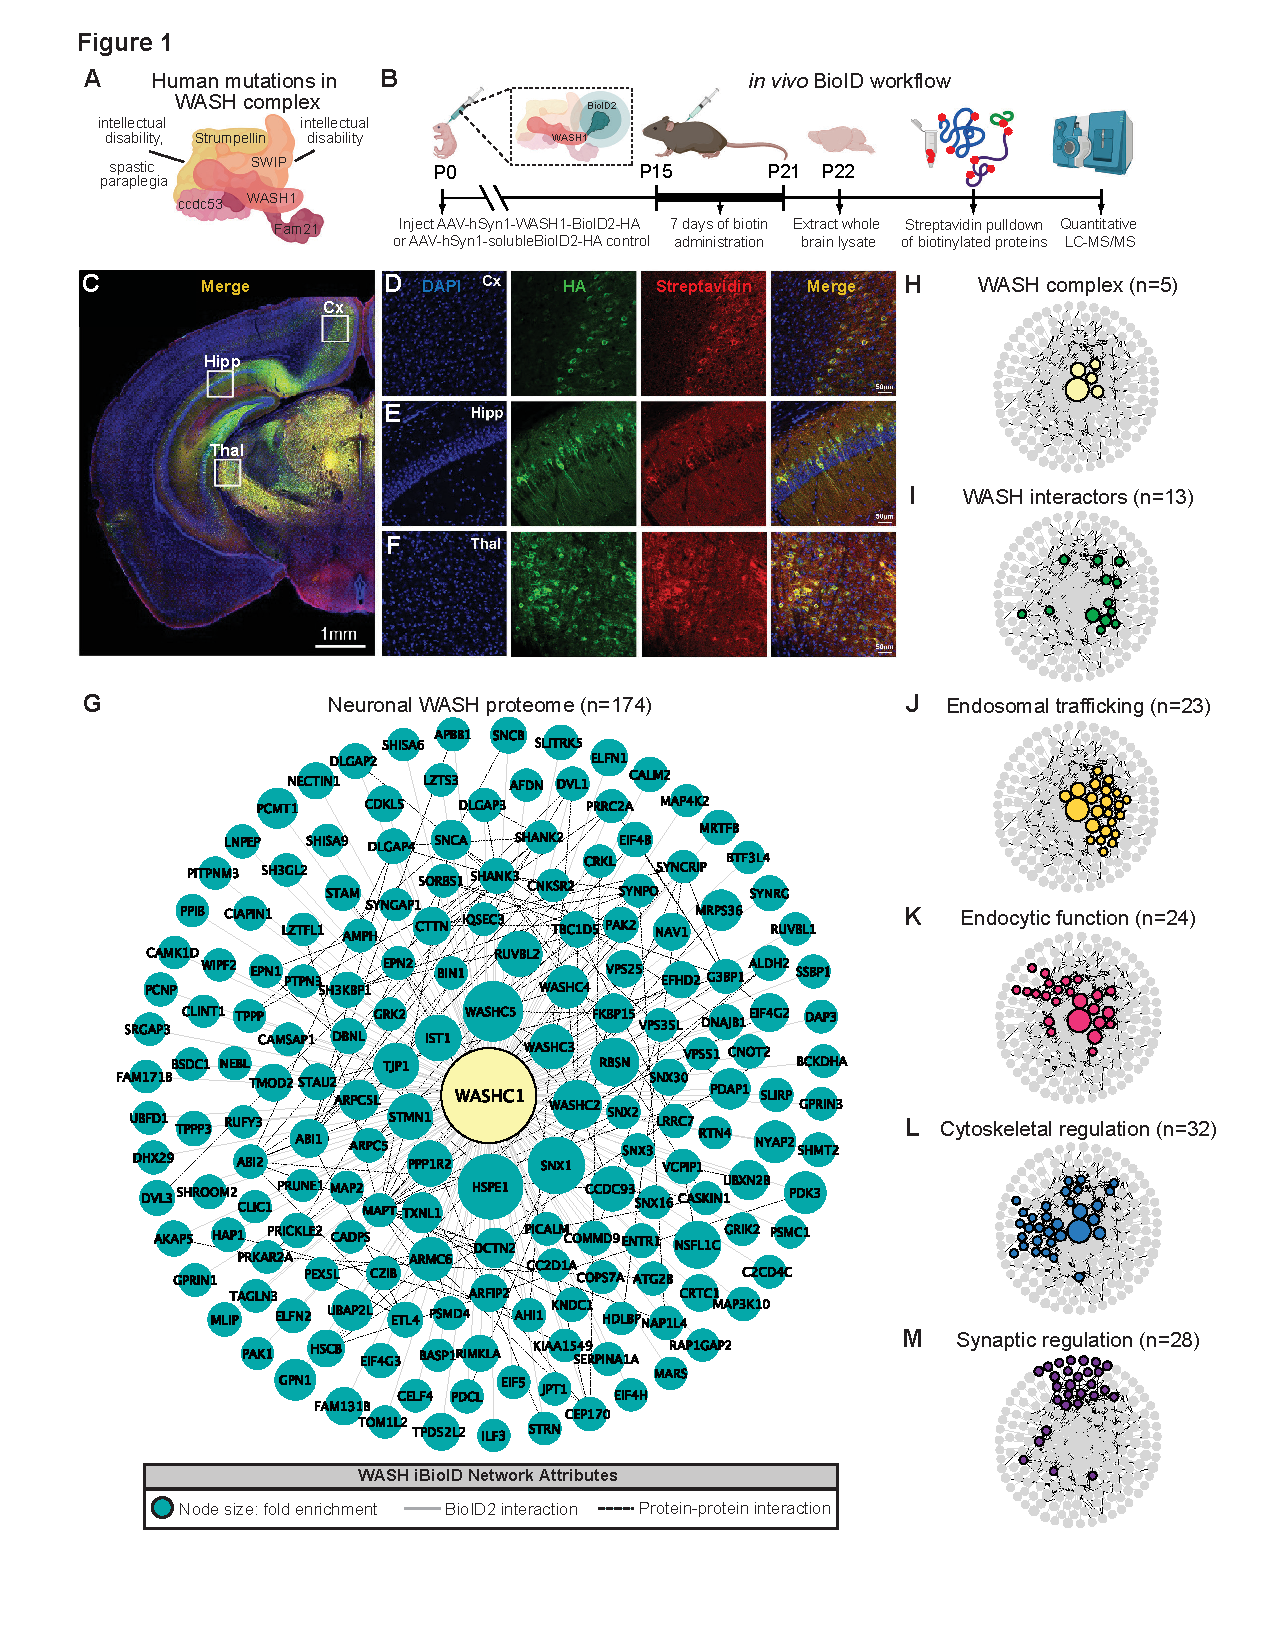
\includegraphics[height=0.5\linewidth, keepaspectratio]{Figure_01}
        \caption{\legend}
	\end{fullwidth}
\end{figure}


%%%%%%%%%%%%%%%%%%%%%%%%%%%%%%%%%%%%%%%%%%%%%%%%%%%%%%%%%%%%
%%% 3. RESULTS
%%%%%%%%%%%%%%%%%%%%%%%%%%%%%%%%%%%%%%%%%%%%%%%%%%%%%%%%%%%%

\section{Results}

% RESULTS

\subsection{Identification of the \textit{in vivo} WASH complex proteome}

While multiple mutations within the WASH complex have been identified in humans 
(Assoum et al., 2020; Elliott et al., 2013; Ropers et al., 2011; 
Valdmanis et al., 2007), how these mutations lead to neurological
dysfunction remains unknown (Figure). Given that previous work in
non-neuronal cultured cells and non-mammalian organisms have established that
the WASH complex functions in endosomal trafficking, we first aimed to determine
whether this role was conserved in the mouse nervous system (Alekhina et al.,
2017; Billadeau et al., 2010; Derivery et al., 2009; Gomez et al., 2012; Gomez
and Billadeau, 2009). To discover the likely molecular functions of the neuronal
WASH complex, we utilized an in vivo BioID (iBioID) paradigm developed in our
laboratory to identify the WASH complex proteome from brain tissue (Uezu et al.,
2016). BioID probes were generated by fusing a component of the WASH complex,
WASH1 (gene: Washc1), with the promiscuous biotin ligase, BioID2 (WASH1-BioID2,
Figure 1B), or by expressing BioID2 alone (negative control, solubleBioID2)
under the neuron-specific, human Synapsin-1 promoter (Kim et al., 2016). We
injected adenoviruses (AAV) expressing these constructs into the cortex of
wild-type postnatal day zero (P0) mice \textbf{(Figure 1B)}. Two weeks post-injection, we
administered daily subcutaneous biotin for seven days to biotinylate in vivo
substrates. The viruses displayed efficient expression and activity in brain
tissue, as evidenced by colocalization of the WASH1-BioID2 viral epitope (HA)
and biotinylated proteins (Streptavidin) \textbf{(Figures 1C-F)}. For label-free
quantitative high-mass accuracy LC-MS/MS analyses, whole brain samples were
collected at P22, snap-frozen, and processed as previously described (Uezu et
al., 2016). A total of 2,311 proteins were identified across all three
experimental replicates, which were further analyzed for those with significant
enrichment in WASH1-BioID2 samples over solubleBioID2 negative controls 
\textbf{(Table S1)}. 

%-------------------------------------------------------------------------------
% Figure 1.
%-------------------------------------------------------------------------------

%\begin{figure}
%\begin{fullwidth}
%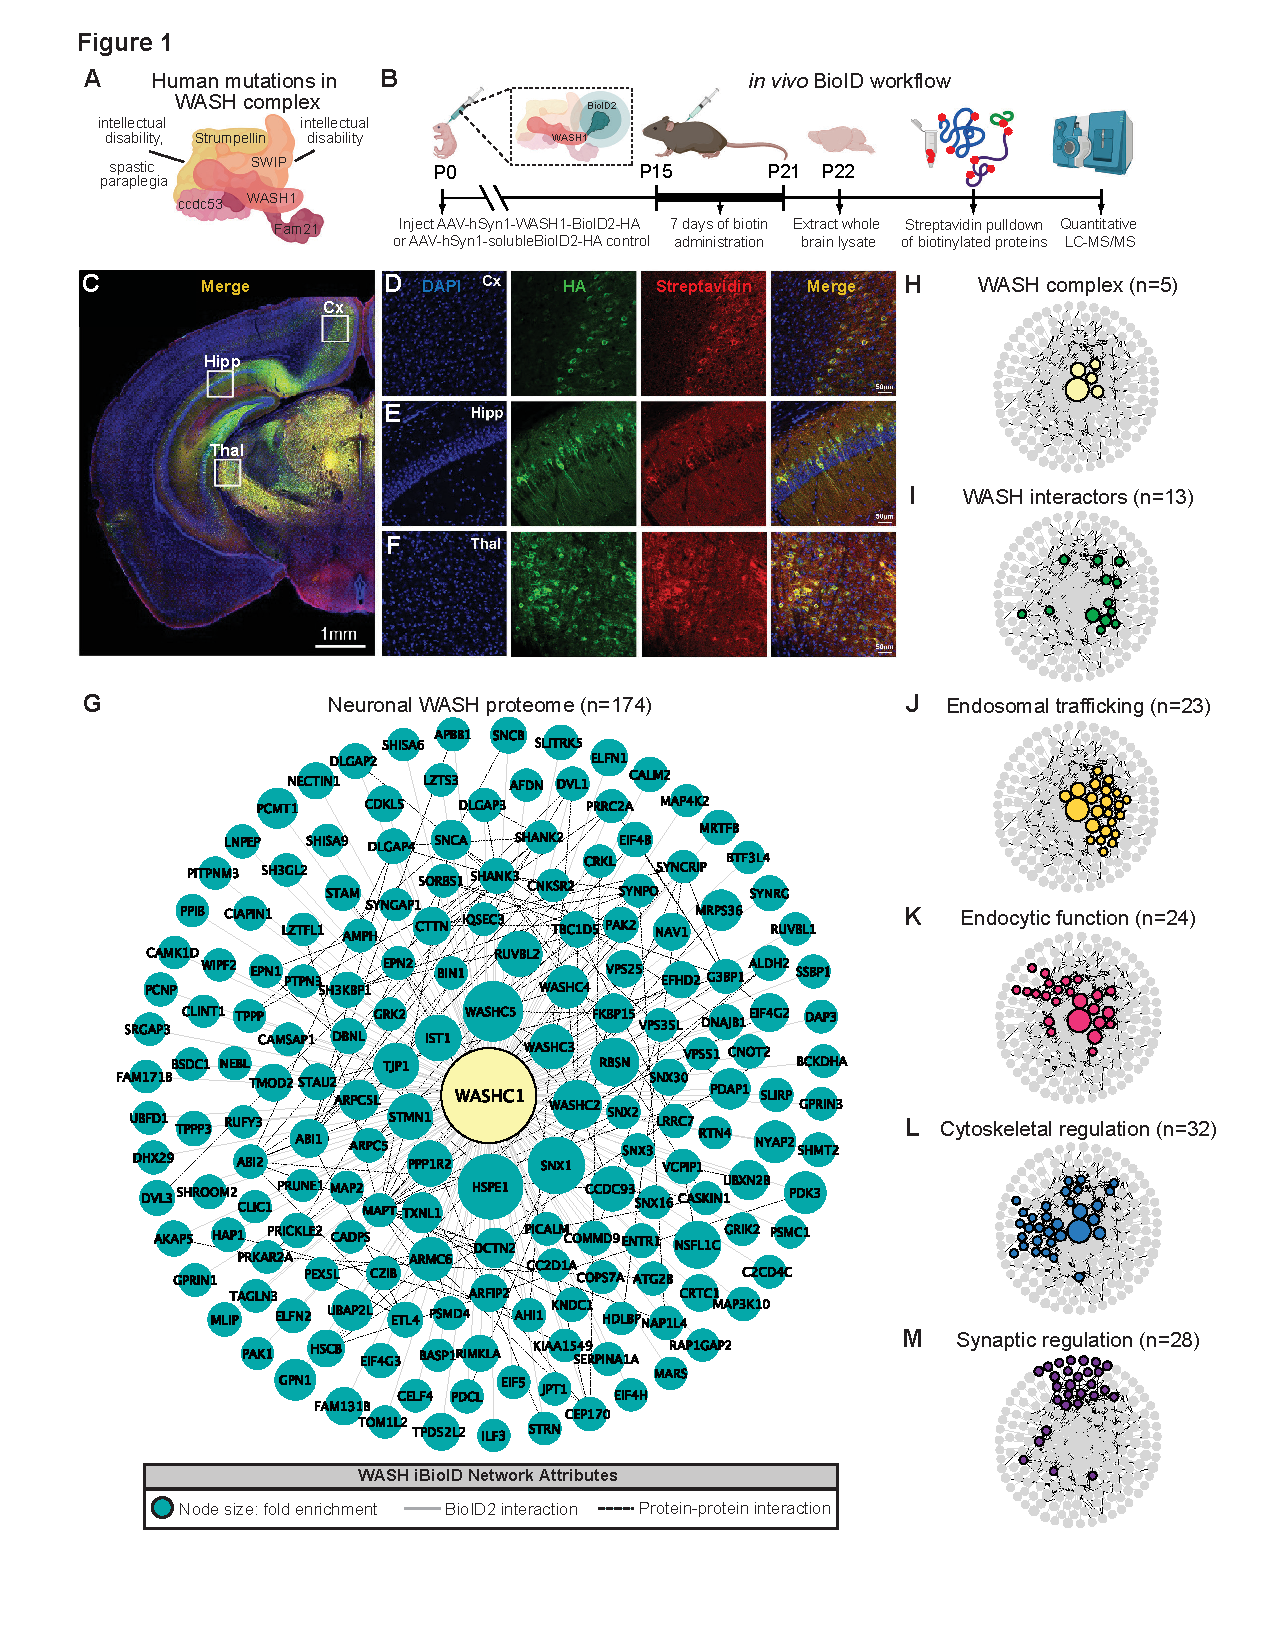
\includegraphics[width=0.95\linewidth, keepaspectratio]{Figure_01}
%	\caption{ \textbf{Identification of the WASH complex proteome in vivo confirms a
%	neuronal role in endosomal trafficking.}
%	(A) The WASH complex is composed of five subunits, Washc1 (WASH1), Washc2
%	(FAM21), Washc3 (CCDC53), Washc4 (SWIP), and Washc5 (Strumpellin). Human
%	mutations in these components are associated with spastic paraplegia (De Bot et
%	al., 2013; Jahic et al., 2015; Valdmanis et al., 2007), Ritscher-Schinzel
%	Syndrome (Elliott et al., 2013), and intellectual disability (Assoum et al.,
%	2020; Ropers et al., 2011). 
%	(B) A BioID2 probe was attached to the c-terminus of WASH1 and expressed under
%	the human synapsin-1 (hSyn1) promoter in an AAV construct for in vivo BioID
%	(iBioID). iBioID probes (WASH1-BioID2-HA, or negative control solubleBioID2-HA)
%	were injected into wild-type mouse brain at P0 and allowed to express for two
%	weeks. Subcutaneous biotin injections (24 mg/kg) were administered over seven
%	days for biotinylation, and then brains were harvested for isolation and
%	purification of biotinylated proteins. LC-MS/MS identified proteins
%	significantly enriched in all three replicates of WASH1-BioID2 samples over
%	soluble-BioID2 controls. 
%	(C) Representative image of WASH1-BioID2-HA expression in a mouse coronal brain
%	section (Cx = cortex, Hipp = hippocampus, Thal = thalamus). Scale bar, 1 mm.
%	(D) Representative image of WASH1-BioID2-HA expression in mouse cortex (inset
%	from C). Individual panels show nuclei (DAPI, blue), AAV construct HA epitope
%	(green), and biotinylated proteins (Streptavidin, red). Merged image shows
%	colocalization of HA and Streptavidin (yellow). Scale bar, 50 µm. 
%	(E) Representative image of WASH1-BioID2-HA expression in mouse hippocampus
%	(inset from C). Scale bar, 50 µm.
%	(F) Representative image of WASH1-BioID2-HA expression in mouse thalamus (inset
%	from C). Scale bar, 50 µm.
%	(G) iBioID identified known and unknown proteins interactors of the WASH complex
%	in murine neurons. Nodes size represents protein abundance fold-enrichment over
%	negative control (range: 3 to 181.7), solid grey edges delineate iBioID
%	interactions between the WASHC1 probe (seen in yellow at the center) and
%	identified proteins, dashed edges indicate known protein-protein interactions
%	from HitPredict database (López et al., 2015). (H-I) Clustergrams of: 
%	(H) All five WASH complex proteins identified by iBioID.
%	(I) Previously reported WASH interactors (13/174), including the CCC and
%	Retriever complexes.
%	(J) Endosomal trafficking proteins (23/174 proteins).
%	(K) Endocytic proteins (24/174).
%	(L) Proteins involved in cytoskeletal regulation (32/174), including Arp2/3
%	subunit ARPC5.
%	(M) Synaptic proteins (28/174). Clustergrams were annotated by hand and
%	cross-referenced with Metascape (Zhou et al., 2019) GO enrichment of WASH1
%	proteome constituents over all proteins identified in the BioID experiment.
%	}
%\label{fig:Figure_01}
%\end{fullwidth}
%\end{figure}

%-------------------------------------------------------------------------------

The resulting neuronal WASH proteome included 174 proteins that were
significantly enriched (Fold-change $\geq$ 3.0, Benjamini-Hochberg P-Adjust $<$ 0.1,
\textbf{Figure 1G}). Of these proteins, we identified all five WASH complex components
\textbf{(Figure 1H)}, as well as 13 previously reported WASH complex interactors 
\textbf{(Figure 1I)} (McNally et al., 2017; Phillips-Krawczak et al., 2015; Simonetti and
Cullen, 2019; Singla et al., 2019), which provided strong validity for our
proteomic approach and analyses. Additional bioinformatic analyses of the
neuronal WASH proteome identified a network of proteins implicated in vesicular
trafficking, including 23 proteins enriched for endosomal functions \textbf{(Figure 1J)}
and 24 proteins enriched for endocytic functions \textbf{(Figure 1K)}. Among these
endosomal and endocytic proteins were components of the recently identified
endosomal sorting complexes, CCC (CCDC93 and COMMD9) and Retriever (VPS35L)
(Phillips-Krawczak et al., 2015; Singla et al., 2019), as well as multiple
sorting nexins important for recruitment of trafficking regulators to the
endosome and cargo selection, such as SNX1-3, and SNX16 (Kvainickas et al.,
2017; Maruzs et al., 2015; Simonetti et al., 2017). These data demonstrated that
the WASH complex interacts with many of the same proteins in neurons as it does
in yeast, amoebae, flies, and mammalian cell lines. Furthermore, there were 32
proteins enriched for cytoskeletal regulatory functions \textbf{(Figure 1L)}, including
actin-modulatory molecules such as the Arp2/3 complex subunit ARPC5, which is
consistent with WASH’s role in activating this complex to stimulate actin
polymerization at endosomes for vesicular scission (Billadeau et al., 2010;
Derivery et al., 2009). The WASH1-BioID2 isolated complex also contained 28
proteins known to localize to the excitatory post-synapse \textbf{(Figure 1M)}. This
included many core synaptic scaffolding proteins, such as SHANK2-3 and DLGAP2-4
(Chen et al., 2011; Mao et al., 2015; Monteiro and Feng, 2017; Wan et al.,
2011), as well as modulators of synaptic receptors such as SYNGAP1 and SHISA6
(Barnett et al., 2006; Clement et al., 2012; Kim et al., 2003; Klaassen et al.,
2016), which was consistent with the idea that vesicular trafficking plays an
important part in synaptic function and regulation. Taken together, these
results support a major endosomal trafficking role of the WASH complex in mouse
brain. 

\subsection{The SWIP\textsuperscript{P1019R} mutation destabilizes the WASH complex}

To determine how disruption of the WASH complex may lead to
disease, we generated a mouse model of a human missense mutation found in
children with intellectual disability, WASHC4\textsuperscript{c.3056c>g} 
(protein: SWIP\textsuperscript{P1019R}) (Ropers et al., 2011). 
Due to the sequence homology of human and mouse Washc4
genes, we were able to introduce the same point mutation in exon 29 of murine
Washc4 using CRISPR (Derivery and Gautreau, 2010; Ropers et al., 2011). This C>G
point mutation results in a Proline>Arginine substitution at position 1019 of
SWIP’s amino acid sequence \textbf{(Figure 2A)}, a region thought to be critical for its
binding to the WASH component, Strumpellin (Jia et al., 2010; Ropers et al.,
2011). Western blot analysis of brain lysate from adult homozygous SWIP\textsuperscript{P1019R}
mutant mice (referred to from here on as MUT mice) displayed significantly
decreased abundance of two WASH complex members, Strumpellin and WASH1 
\textbf{(Figure 2B)}. These results phenocopied data from the human patients (Ropers et al.,
2011) and suggested that the WASH complex is unstable in the presence of this
SWIP point mutation in vivo. To test whether this mutation disrupted
interactions between WASH complex subunits, we compared the ability of wild-type
SWIP (WT) and SWIP\textsuperscript{P1019R} (MUT) to co-immunoprecipitate with Strumpellin and
WASH1 in HEK cells. Compared to WT, MUT SWIP co-immunoprecipitated significantly
less Strumpellin and WASH1 (IP: 54.8\% and 41.4\% of WT SWIP, respectively),
suggesting that the SWIP\textsuperscript{P1019R} mutation hinders WASH complex formation 
\textbf{(Figure 2 and Figure Supplement 1)}. Together these data support the notion that 
SWIP\textsuperscript{P1019R} is a damaging mutation that not only impairs its function, 
but also results in significant reductions of the WASH complex as a whole.

\subsection{Spatial proteomics analysis of SWIP\textsuperscript{P1019R} mutant mouse brain}

Next, we aimed to understand the impact of the SWIP\textsuperscript{P1019R} mutation on the
subcellular organization of the mouse brain proteome. We performed spatial
proteomics by following the protocol established by Geladaki \textit{et al.}, with
modifications for homogenization of brain tissue (Geladaki et al., 2019; Hallett
et al., 2008). We isolated seven subcellular fractions from brain tissue and
quantified proteins in these samples using 16-plex TMT proteomics. Using this
spatial proteomics dataset, we developed a data-driven clustering approach to
classify proteins into subcellular compartments. This approach, which differs
from the support vector machine learning algorithm employed by Geladaki et al.
(2019), was motivated by the lack of a large corpus of brain-specific protein
subcellular localization information, and the greater complexity of brain tissue
compared to cultured cells. In addition to evaluating differential protein
abundance between WT and SWIP\textsuperscript{P1019R} MUT brain, we utilized this spatial
proteomics dataset to analyze network-level changes in groups of covarying
proteins to better understand WASH’s function and explore the cellular
mechanisms by which SWIP\textsuperscript{P1019R} causes disease. 

Brains from 10-month-old mice were gently homogenized to release intact
organelles, followed by successive centrifugation steps to enrich subcellular
compartments into different fractions based on their density \textbf{(Figure 2C)}
(Geladaki et al., 2019). Seven WT and seven MUT fractions (each prepared from
one brain, 14 samples total) were labeled with unique isobaric tandem-mass tags
and concatenated. We also included two sample pooled quality controls (SPQCs),
which allowed us to assess experimental variability and perform normalization
between experiments. By performing this experiment in triplicate, deep coverage
of the mouse brain proteome was obtained—across all 48 samples we quantified
86,551 peptides, corresponding to 7,488 proteins. After data pre-processing,
normalization, and filtering we retained 5,897 reproducibly quantified proteins
in the final dataset \textbf{(Table S2)}. 

We used generalized linear models (GLMs) to assess differential protein
abundance for intra-fraction comparisons between WT and MUT genotypes, and for
overall comparisons between WT and MUT groups, adjusted for baseline differences
in subcellular fraction. In the first analysis, there were 85 proteins with
significantly altered abundance in at least one of the 7 subcellular fractions
(Benjamini-Hochberg P-Adjust $<$ 0.1, \textbf{Table S2} and 
\textbf{Figure 2 Supplement 2}). Five proteins were differentially abundant 
between WT and MUT in all 7 fractions, including four WASH proteins 
and RAB21A—a known WASH interactor that functions in early endosomal 
trafficking (WASHC1, WASHC2, WASHC4, WASHC5, \textbf{Figure 2E}) 
(Del Olmo et al., 2019; Simpson et al., 2004). The abundance of the
remaining WASH complex protein, WASHC3, was found to be very low and was not
retained in the final dataset due to its sparse quantification. These data
affirm that the SWIP\textsuperscript{P1019R} mutation destabilizes the WASH complex. Next, to
evaluate global differences between WT and MUT brain, we analyzed the average
effect of genotype on protein abundance across all fractions. At this level,
there were 687 differentially abundant proteins between WT and MUT brain
(Bonferroni P-Adjust $<$ 0.05) \textbf{(Table S2)}. We then aimed to place these
differentially abundant proteins into a more meaningful biological context using
a systems-based approach.

For network-based analyses, we clustered the protein covariation network defined
by pairwise correlations between all 5,897 proteins. Our data-driven,
quality-based approach used Network Enhancement (Wang et al., 2018) to remove
biological noise from the covariation network and employed the Leiden algorithm
(Traag et al., 2019) to identify optimal partitions of the graph. We enforced
module quality by permutation testing (Ritchie et al., 2016) to ensure that
identified modules exhibited a non-random topology. Clustering of the protein
covariation graph identified 255 modules of proteins that strongly covaried
together (see Methods for complete description of clustering approach). 
To test for module-level differences between WT and MUT brain, we summarized
modules for each biological replicate (a single subcellular fraction prepared
from either a WT or MUT mouse) as the sum of their proteins, and extended our
GLM framework to identify changes in module abundance (adjusted for fraction
differences) between genotypes. 37 of the 255 modules exhibited significant
differences in WT versus MUT brain (Bonferroni P-Adjust $<$ 0.05; \textbf{Table S3}). 
Of note, the module containing the WASH complex, M19, was predicted to have
endosomal function by annotation of protein function, and was enriched for
proteins identified by WASH1-BioID2 (hypergeometric test P-Adjust $<$ 0.05, bold
node edges, \textbf{Figure 2D}). Similar to the WASH iBioID proteome \textbf{(Figure 1)}, M19
contained components of the CCC (CCDC22, CCDC93, COMMD1-3, COMMD6-7, and COMMD9)
and Retriever sorting complexes (VPS26C and VPS35L), but not the Retromer
sorting complex, suggesting that in the brain, the WASH complex may not interact
as closely with Retromer as it does in other cells \textbf{(Figure 2D)}. Across all
fractions, the abundance of M19 was significantly lower in MUT brain compared to
WT, providing evidence that the SWIP\textsuperscript{P1019R} mutation reduces the stability of
this protein subnetwork and impairs its function \textbf{(Figure 2F-G)}. 

In contrast to the decreased abundance of the WASH complex/endosome module, M19,
we observed three modules (M2, M159, and M213) which were enriched for lysosomal
protein components (Geladaki et al., 2019), and exhibited increased abundance in
MUT brain \textbf{(Figure 3)}. M159 \textbf{(Figure 3B)} contained the lysosomal protease
Cathepsin A (CTSA), while M213 \textbf{(Figure 3D)} contained Cathepsin B (CTSB), as well
as two key lysosomal hydrolases GLB1 and MAN2B2, and M2 \textbf{(Figure 3C)} contained
two Cathepsins (CTSS and CTSL) and several lysosomal hydrolases (e.g. GNS, GLA,
and MAN2B1) (Eng and Desnick, 1994; Mayor et al., 1993; Mok et al., 2003; Moon
et al., 2016; Patel et al., 2018; Regier and Tifft, 1993; Rosenbaum et al.,
2014). Notably, M2 also contained the lysosomal glycoprotein progranulin (GRN),
which is integral to proper lysosome function and whose loss is widely linked
with neurodegenerative pathologies (Baker et al., 2006; Pottier et al., 2016;
Tanaka et al., 2017; Zhou et al., 2018). In addition, M2 contained the hydrolase
IDS, whose loss causes a lysosomal storage disorder that can present with
neurological symptoms (Hopwood et al., 1993; Schröder et al., 1994). The overall
increase in abundance of modules M2, M159, and M213, and these key lysosomal
proteins (Figure 3E-G), may therefore reflect an increase in flux through
degradative lysosomal pathways in SWIP\textsuperscript{P1019R} brain. 

Furthermore, Module 2 \textbf{(Figure 3C)} included multiple membrane proteins and
extracellular proteins, such as ITGA5 (an integrin shown to be upregulated and
redistributed upon loss of WASH1), ATP13A2 (a cation transporter whose loss
causes a Parkinsonian syndrome), and MMP17 (an extracellular metalloprotease),
suggesting a link between these proteins and lysosomal enzymatic function
(English et al., 2000; Ramirez et al., 2006; Zech et al., 2011). Increased
abundance of these M2 proteins in MUT brain may indicate that WASH complex
disruption alters their cellular localization. Taken together, these changes
appear to reflect a pathological condition characterized by distorted lysosomal
metabolism and altered cellular trafficking.

In addition to these endo-lysosomal changes, network alterations were
evident for an endoplasmic reticulum (ER) module (M83), supporting a shift in
the proteostasis of mutant neurons \textbf{(Figure 2 and Figure Supplement 3B)}. Notably,
within the ER module, M83, there was increased abundance of chaperones (e.g.
HSPA5, PDIA3, PDIA4, PDIA6, and DNAJC3) that are commonly engaged in presence of
misfolded proteins (Bartels et al., 2019; Kim et al., 2020; Montibeller and de
Belleroche, 2018; Synofzik et al., 2014; Wang et al., 2016). This elevation of
ER stress modulators can be indicative of neurodegenerative states, in which the
unfolded protein response (UPR) is activated to resolve misfolded species
(Garcia-Huerta et al., 2016; Hetz and Saxena, 2017). These data demonstrate that
loss of WASH function not only alters endo-lysosomal trafficking, but also
causes increased stress on cellular homeostasis. 
Finally, besides these endo-lysosomal and homeostatic changes, we also observed
two synaptic modules (M35 and M248) that were reduced in MUT brain \textbf{(Figure
2 and Figure Supplement 3C-D)}. These included mostly excitatory post-synaptic
proteins such as HOMER2 and DLG4 (also identified in WASH1-BioID, \textbf{Figure 1}),
consistent with endosomal WASH influencing synaptic regulation. Decreased
abundance of these modules indicates that loss of the WASH complex may result in
failure of these proteins to be properly trafficked to the synapse.

\subsection{SWIP mutant neurons display endo-lysosomal structural abnormalities}

Combined, the proteomics data strongly suggested that endo-lysosomal
pathways are altered in adult SWIP\textsuperscript{P1019R} mutant mouse brain. Next, we analyzed
whether structural changes in this system were evident in primary neurons.
Cortical neurons from littermate WT and MUT P0 pups were cultured for 15 days in
vitro (DIV15, Figure 4A), then fixed and stained for established markers of
early endosomes (Early Endosome Antigen 1, EEA1; Figures 4B and 4C) and
lysosomes (Cathepsin D, CathD; Figures 4D and 4E). Reconstructed
three-dimensional volumes of EEA1 and Cathepsin D puncta revealed that MUT
neurons display larger EEA1+ somatic puncta than WT neurons (Figures 4G and 4J),
but no difference in the total number of EEA1+ puncta (Figure 4F). This finding
is consistent with a loss-of-function mutation, as loss of WASH activity
prevents cargo scission from endosomes and leads to cargo accumulation (Bartuzi
et al., 2016; Gomez et al., 2012). Conversely, MUT neurons exhibited
significantly less Cathepsin D+ puncta than WT neurons (Figure 4H), but the
remaining puncta were significantly larger than those of WT neurons (Figures 4I
and 4K). These data support the finding that the SWIP\textsuperscript{P1019R} mutation results in
both molecular and morphological abnormalities in the endo-lysosomal pathway.

\subsection{SWIP\textsuperscript{P1019R} mutant brains exhibit 
lipofuscin accumulation and markers of cell death}

As there is strong evidence that dysfunctional endo-lysosomal trafficking 
and elevated ER stress are associated with neurodegenerative disorders, 
adolescent (P42) and adult (10 month-old, 10mo) WT and MUT brain tissue 
were analyzed for the presence of cleaved caspase-3, a marker of apoptotic 
pathway activation, in four brain regions (Boatright and Salvesen, 2003; 
Porter and Jänicke, 1999). Very little cleaved caspase-3
staining was present in WT and MUT mice at adolescence (Figures 5A, 5B, and
Figure 5-figure supplement 1). However, at 10mo, the MUT motor cortices
displayed significantly greater cleaved caspsase-3 staining compared to
age-matched WT littermate controls (Figures 5D, 5E, and 5H). Furthermore, this
difference appeared to be selective for the motor cortex, as we did not observe
significant differences in cleaved caspase-3 staining at either age for
hippocampal, striatal, or cerebellar regions (Figure 5-figure supplement 1).
These data suggested that neurons of the motor cortex were particularly
susceptible to disruption of endo-lysosomal pathways downstream of SWIP\textsuperscript{P109R},
perhaps because long-range corticospinal projections require high fidelity of
trafficking pathways (Blackstone et al., 2011; Slosarek et al., 2018; Wang et
al., 2014). 

To further examine the morphology of primary motor cortex neurons at a
subcellular resolution, samples from age-matched 7-month-old WT and MUT mice
(7mo, 3 animals each) were imaged by transmission electron microscopy (TEM).
Strikingly, we observed large electron-dense inclusions in the cell bodies of
MUT neurons (arrows, Figure 5L; pseudo-colored region, 5N). These dense
structures were associated electron-lucent lipid-like inclusions (asterisk,
Figure 5N), and were visually consistent with lipofuscin accumulation at
lysosomal residual bodies (Poët et al., 2006; Valdez et al., 2017; Yoshikawa et
al., 2002). Lipofuscin is a by-product of lysosomal breakdown of lipids,
proteins, and carbohydrates, which naturally accumulates over time in
non-dividing cells such as neurons (Höhn and Grune, 2013; Moreno-García et al.,
2018; Terman and Brunk, 1998). However, excessive lipofuscin accumulation is
thought to be detrimental to cellular homeostasis by inhibiting lysosomal
function and promoting oxidative stress, often leading to cell death (Brunk and
Terman, 2002; Powell et al., 2005). As a result, elevated lipofuscin is
considered a biomarker of neurodegenerative disorders, including Alzheimer’s
disease, Parkinson’s disease, and Neuronal Ceroid Lipofuscinoses (Moreno-García
et al., 2018). Therefore, the marked increase in lipofuscin area and number seen
in MUT electron micrographs (Figures 5O and 5P, respectively) is consistent with
the increased abundance of lysosomal pathways observed by proteomics, and likely
reflects an increase in lysosomal breakdown of cellular material. Together these
data indicate that SWIP\textsuperscript{P1019R} results in pathological lysosomal function that
could lead to neurodegeneration. 

\subsection{SWIP\textsuperscript{P1019R} mutant mice display persistent deficits 
in cued fear memory recall}

To observe the functional consequences of the SWIP\textsuperscript{P1019R} mutation, we next
studied WT and MUT mouse behavior. Given that children with homozygous
SWIP\textsuperscript{P1019R} point mutations display intellectual disability (Ropers et al., 2011)
and SWIP\textsuperscript{P1019R} mutant mice exhibit endo-lysosomal disruptions implicated in
neurodegenerative processes, behavior was assessed at two ages: adolescence
(P40-50), and mid-late adulthood (5.5-6.5 mo). Interestingly, MUT mice performed
equivalently to WT mice in episodic and working memory paradigms, including
novel object recognition and Y-maze alternations (Figure 6-figure supplement 1).
However, in a fear conditioning task, MUT mice displayed a significant deficit
in cued fear memory (Figure 6). This task tests the ability of a mouse to
associate an aversive event (a mild electric footshock) with a paired tone
(Figure 6A). Freezing behavior of mice during tone presentation is attributed to
hippocampal or amygdala-based fear memory processes (Goosens and Maren, 2001;
Maren and Holt, 2000; Vazdarjanova and McGaugh, 1998). Forty-eight hours after
exposure to the paired tone and footshock, MUT mice showed a significant
decrease in conditioned freezing to tone presentation compared to their WT
littermates (Figures 6B and 6C). To ensure that this difference was not due to
altered sensory capacities of MUT mice, we measured the startle response of mice
to both electric foot shock and presented tones. In line with intact sensation,
MUT mice responded comparably to WT mice in these tests (Figure 6-figure
supplement 2). These data demonstrate that although MUT mice perceive footshock
sensations and auditory cues, it is their memory of these paired events that is
significantly impaired. Additionally, this deficit in fear response was evident
at both adolescence and adulthood (top panels, and bottom panels, respectively,
Figures 6B and 6C). These changes are consistent with the hypothesis that
SWIP\textsuperscript{P1019R} is the cause of cognitive impairments in humans. 

\subsection{SWIP\textsuperscript{P1019R} mutant mice exhibit surprising motor 
deficits that are confirmed in human patients}

Because SWIP\textsuperscript{P1019R} results in endo-lysosomal pathology
consistent with neurodegenerative disorders in the motor cortex, we next
analyzed motor function of the mice over time. First, we tested the ability of
WT and MUT mice to remain on a rotating rod for five minutes (Rotarod, Figures
7A-7C). At both adolescence and adulthood, MUT mice performed markedly worse
than WT littermate controls (Fig 7C). Mouse performance was not significantly
different across trials, which suggested that this difference in retention time
was not due to progressive fatigue, but more likely due to an overall difference
in motor control (Mann and Chesselet, 2015).

To study the animals’ movement at a finer scale, the gait of WT and MUT mice was
also analyzed using a TreadScan system containing a high-speed camera coupled to
a transparent treadmill (Figure 7D) (Beare et al., 2009). Interestingly, while
the gait parameters of mice were largely indistinguishable across genotypes at
adolescence, a striking difference was seen when the same mice were aged to
adulthood (Figures 7E-7G). In particular, MUT mice took slower (Figure 7E),
longer strides (Figure 7F), stepping closer to the midline of their body (track
width, Figure 7- figure supplement 1), and their gait symmetry was altered so
that their strides were no longer perfectly out of phase (out of phase=0.5,
Figure 7G). While these differences were most pronounced in the rear limbs (as
depicted in Figure 7E-7G), the same trends were present in front limbs (Figure
7-figure supplement 1). These findings demonstrate that SWIP\textsuperscript{P1019R} results in
progressive motor function decline that was detectable by the rotarod task at
adolescence, but which became more prominent with age, as both gait and strength
functions deteriorated.

These marked motor findings prompted us to re-evaluate the original reports of
human SWIP\textsuperscript{P1019R} patients (Ropers et al., 2011). While developmental delay or
learning difficulties were the primary impetus for medical evaluation, all
patients also exhibited motor symptoms (mean age = 10.4 years old, Figure 7H).
The patients’ movements were described as “clumsy” with notable fine motor
difficulties, dysmetria, dysdiadochokinesia, and mild dysarthria on clinical
exam (Figure 7H). Recent communication with the parents of these patients, who
are now an average of 21 years old, revealed no notable symptom exacerbation. It
is therefore possible that the SWIP\textsuperscript{P1019R} mouse model either exhibits
differences from human patients or may predict future disease progression for
these individuals, given that we observed significant worsening at 5-6 months
old in mice (which is thought to be equivalent to ~30-35 years old in humans)
(Dutta and Sengupta, 2016; Zhang et al., 2019).

% Table: Clinical findings in human patients.
%\begin{tabularx}{\textwidth}{X|l}
%\textbf{Patient} & \textbf{Age} & \textbf{Sex} & \textbf{Motor Skills} \\
%\hline
%1 & 18 & F & + \\
%\end{tabularx}

%Figure 2. Spatial proteomics and network covariation analysis reveal significant
%disruptions to the WASH complex and an endosomal module in SWIPP1019R mutant
%mouse brain
%(A) Mouse model of the human SWIPP1019R missense mutation created using CRISPR.
%A C>G point mutation was introduced into exon29 of murine Washc4, leading to a
%P1019R amino acid substitution. We hypothesize (H1) that this mutation causes
%instability of the WASH complex.  
%(B) Representative western blot and quantification of WASH components,
%Strumpellin and WASH1 (predicted sizes in kDa: 134 and 72, respectively), as
%well as loading control β-Tubulin (55kDa) from whole adult whole brain lysate
%prepared from SWIP WT (Washc4C/C) and SWIP homozygous MUT (Washc4G/G) mice.  Bar
%plots show quantification of band intensities relative to WT (n=3 mice per
%genotype). Strumpellin (WT 100.0 ± 5.2%, MUT 3.5 ± 0.7%, t2.1=18.44, p=0.0024)
%and WASH1 (WT 100.0 ± 3.8%, MUT 1.1 ± 0.4%, t2.1=25.92, p=0.0013) were
%significantly decreased. Equivalent amounts of protein were analyzed in each
%condition (β-Tubulin: WT 100.0 ± 8.2%, MUT 94.1 ± 4.1%, U=4, p>0.99). 
%(C) Spatial TMT proteomics experimental design. 7 subcellular fractions were
%prepared from one WT and one MUT mouse (10mo). These samples, as well as two
%pooled quality control (QC) samples, were labeled with unique TMT tags and
%concatenated for simultaneous LC-MS/MS analysis. This experiment was repeated
%three times (3 WT and 3 MUT brains total). To detect network-level changes,
%proteins were clustered into modules, and general linearized models (GLMs) were
%used to identify differences in module abundance between WT and MUT samples. The
%network shows an overview of the spatial proteomics graph in which the 37
%differentially abundant modules are indicated by colored nodes. 
%(D) Protein module 19 (M19) contains subunits of the WASH, CCC, and Retriever
%complexes. Node size denotes its weighted degree centrality (~importance in
%module); purple node color indicates proteins with altered abundance in MUT
%brain relative to WT; black node border denotes proteins identified in the
%WASH1-BioID proteome (Figure 1); red, yellow, and green borders highlight
%protein components of the CCC, Retriever, and WASH complexes; black edges
%indicate known protein-protein interactions; and grey-red edges denote the
%relative strength of protein covariation within a module (gray = weak, red =
%strong). P-adjust values represent enrichment of proteins identified in the
%CORUM database adjusted for multiple comparisons (Giurgiu et al., 2019). 
%(E) Difference in normalized protein abundance for four WASH proteins found in
%M19 (SWIP: WT 6.28 ± 0.41, MUT 4.89 ± 0.28, p=3.98x10-28; WASH1: WT 6.41 ± 0.47,
%MUT 4.65 ± 0.62, p=7.92x10-18; FAM21: WT 6.29 ± 0.48, MUT 5.29 ± 0.49,
%p=3.27x10-16; Strumpellin: WT 7.85 ± 0.52, MUT 6.59 ± 0.53, p=9.06x10-25) and
%one control (Tubulin 4a: WT 8.57 ± 0.52, MUT 8.52 ± 0.58, p>0.99) across all
%three experimental replicates (n=3 independent experiments), presented as
%log2(adjusted protein intensities). 
%(F) Normalized average intensities for every protein within M19 across all seven
%subcellular fractions analyzed. Teal lines delineate protein levels in WT
%samples, purple lines delineate protein levels in MUT samples (averaged across
%three experimental replicates). Bolded lines demarcate the fitted intensity
%values for WT and MUT proteins (n=3 independent experiments). 
%(G) Difference in M19 abundance, adjusted for fraction differences and presented
%as log2(adjusted module abundance) (WT 13.21 ± 0.003, MUT 12.99 ± 0.003,
%p=0.0007; n=3 independent experiments). 
%
%Figure 3. Disruption of lysosomal protein networks in SWIPP1019R mutant brain
%(A) Simplified schematic of the endo-lysosomal pathway in neurons. Inset depicts
%representative lysosomal enzymes, such as proteases (CTSA, CTSB, CTSL),
%glycosidases (GLA, GLB1, MAN2B1), and sulfatases (GNS, IDS).  
%(B) Network graph of module 159 (M159). All proteins in M159 exhibit altered
%abundance in MUT brain, including lysosomal proteins, CTSA, PLA2G15, and GM2A. 
%(C) Module 2 (M2) contains multiple lysosomal proteins with increased abundance
%in MUT brain compared to WT, including CTSS, CTSL, GRN, IDS, MAN2B1. 
%(D) Module 213 (M213) contains multiple proteins with increased abundance in MUT
%brain, including lysosomal proteins, GLB1, GNS, CTSB, MAN2B2, and PLBD2. Network
%attributes (B-D): Node size denotes its weighted degree centrality (~importance
%in module),  node color indicates proteins with altered abundance in MUT brain
%relative to WT, purple outline highlight proteins identified as lysosomal in
%(Geladaki et al., 2019), black edges indicate known protein-protein
%interactions, and grey-red edges denote the relative strength of protein
%covariation within a module (gray = weak, red = strong). P-Adjust values
%represent enrichment of proteins identified as lysosomal in Geladaki et al.,
%2019. 
%(E) The overall effect of genotype on M159 module abundance (WT 10.83 ± 0.002,
%MUT 10.94 ± 0.002, p=0.031). 
%(F) The overall effect of genotype on M2 module abundance (WT 13.74 ± 0.001, MUT
%13.85 ± 0.0009, p=0.0006). 
%(G) The overall effect of genotype on M213 abundance (WT 12.17 ± 0.002, MUT
%12.33 ± 0.002, p=0.0037). Data reported as mean ± SEM, error bars are SEM.
%*p<0.05, ** p<0.01, ***p<0.001, empirical Bayes quasi-likelihood F-test with
%Bonferroni correction (E-G).
%
%Figure 4. SWIPP1019R mutant neurons display structural abnormalities in
%endo-lysosomal compartments in vitro 
%(A) Experimental design. Cortices were dissected from P0 pups, and neurons were
%dissociated and cultured on glass coverslips for 15 days. Cultures were fixed,
%stained, and imaged using confocal microscopy. 3D puncta volumes were
%reconstructed from z-stack images using Imaris software. 
%(B-C) Representative 3D reconstructions of WT and MUT DIV15 neurons
%(respectively) stained for EEA1 (yellow) and MAP2 (magenta). 
%(D-E) Representative 3D reconstructions of WT and MUT DIV15 neurons
%(respectively) stained for Cathepsin D (cyan) and MAP2 (magenta). 
%(F) Graph of the average number of EEA1+ volumes per soma in each image (WT 95.0
%± 5.5, n=24 neurons; MUT 103.7 ± 3.7, n=24 neurons; t40.2=1.314, p=0.1961). 
%(G) Graph of the average EEA1+ volume size per soma shows larger EEA1+ volumes
%in MUT neurons (WT 0.15 ± 0.01 µm3, n=24 neurons; MUT 0.30 ± 0.02 µm3, n=24
%neurons; U=50, p<0.0001). 
%(H) Graph of the average number of Cathepsin D+ volumes per soma illustrates
%less Cathepsin D+ volumes in MUT neurons (WT 30.4 ± 1.4, n=42; MUT 17.2 ± 0.9,
%n=42; t71=7.943, p<0.0001). 
%(I) Graph of the average Cathepsin D+ volume size per soma demonstrates larger
%Cathepsin D+ volumes in MUT neurons (WT 0.54 ± 0.02 µm3, n=42; MUT 0.69 ± 0.04
%µm3, n=42; t63=3.701, p=0.0005). 
%(J) Histogram of EEA1+ volumes illustrate differences in size distributions
%between MUT and WT neurons. 
%(K) Histogram of CathD+ volumes show differences in size distributions between
%MUT and WT neurons. Analyses included at least three separate culture
%preparations. Scale bars, 5 µm (B-E). Data reported as mean ± SEM, error bars
%are SEM. ***p<0.001, ****p<0.0001, two-tailed t-tests or Mann-Whitney U test
%(G).
%
%Figure 5. SWIPP1019R mutant brains exhibit markers of abnormal endo-lysosomal
%structures and cell death in vivo
%(A-B) Representative images of adolescent (P42) WT and MUT motor cortex stained
%with cleaved caspase-3 (CC3, green).
%(C) Anatomical representation of mouse brain with motor cortex highlighted in
%red, adapted from the Allen Brain Atlas (Oh et al., 2014). 
%(D-E) Representative image of adult (10 mo) WT and MUT motor cortex stained with
%CC3 (green).  
%(F, G, I, and J) DAPI co-stained images for (A, B, D, and E, respectively).
%Scale bar for (A-J), 15 µm. 
%(H) Graph depicting the normalized percentage of DAPI+ nuclei that are positive
%for CC3 per image. No difference is seen at P42, but the amount of CC3+ nuclei
%is significantly higher in aged MUT mice (P42 WT 6.97 ± 0.80%, P42 MUT 5.26 ±
%0.90%, 10mo WT 25.38 ± 2.05%, 10mo MUT 44.01 ± 1.90%, H=74.12, p<0.0001). We
%observed no difference in number of nuclei per image between genotypes. 
%(K) Representative transmission electron microscopy (TEM) image taken of soma
%from adult (7mo) WT motor cortex. Arrowheads delineate electron-dense lipofuscin
%material, Nuc = nucleus. 
%(L) Representative transmission electron microscopy (TEM) image taken of soma
%from adult (7mo) MUT motor cortex. 
%(M) Inset from (K) highlights lysosomal structure in WT soma. Pseudo-colored
%region depicts lipofuscin area, demarcated as L. 
%(N) Inset from (L) highlights large lipofuscin deposit in MUT soma (L,
%pseudo-colored region) with electron-dense and electron-lucent lipid-like
%(asterisk) components. 
%(O) Graph of areas of electron-dense regions of interest (ROI) shows increased
%ROI size in MUT neurons (WT 2.4x105 ± 2.8x104 nm2, n=50 ROIs; MUT 8.2x105 ± 9.7
%x104 nm2, n=75 ROIs; U=636, p<0.0001). 
%(P) Graph of the average number of presumptive lysosomes with associated
%electron-dense material reveals increased number in MUT samples (WT 3.14 ± 0.72
%ROIs, n=14 images; MUT 10.86 ± 1.42 ROIs, n=14 images; U=17, p<0.0001). For (N)
%and (O), images were taken from multiple TEM grids, prepared from n=3 animals
%per genotype. Scale bar for all TEM images, 1 µm. Data reported as mean ± SEM,
%error bars are SEM. ***p<0.001, ****p<0.0001, Kruskal-Wallis test (F),
%Mann-Whitney U test (O-P).
%
%Figure 6. SWIPP1019R mutant mice display persistent deficits in cued fear memory
%recall 
%(A) Experimental fear conditioning paradigm. After acclimation to a conditioning
%chamber, mice received a mild aversive 0.4mA footshock paired with a 2900Hz
%tone. 48 hours later, the mice were placed in a chamber with different tactile
%and visual cues. The mice acclimated for two minutes and then the 2900Hz tone
%was played (no footshock) and freezing behavior was assessed. 
%(B) Line graphs of WT and MUT freezing response during cued tone memory recall.
%Data represented as average freezing per genotype in 30 s time bins. The tone is
%presented after t = 120 s, and remains on for 120 seconds (Tone ON). Two
%different cohorts of mice were used for age groups P42 (top) and 6.5mo (bottom).
%Two-way ANOVA analysis of average freezing during Pre-Tone and Tone periods
%reveal a Genotype x Time effect at P42 (WT n=10, MUT n=10, F1,18=4.944,
%p=0.0392) and 6.5mo (WT n=13, MUT n=11, F1,22= 13.61, p=0.0013). 
%(C) Graphs showing the average %time freezing per animal before and during tone
%presentation. Top: freezing is reduced by 20% in MUT adolescent mice compared to
%WT littermates (Pre-tone WT 16.5 ± 2.2%, n=10; Pre-tone MUT 13.0 ± 1.8%, n=10;
%t36=0.8569, p=0.6366; Tone WT 52.8 ± 3.8%, n=10; Tone MUT 38.0 ± 3.6%, n=10;
%t36=3.539, p=0.0023), Bottom: freezing is reduced by over 30% in MUT adult mice
%compared to WT littermates (Pre-tone WT 21.1 ± 2.7%, n=13; Pre-tone MUT 23.7 ±
%3.8%, n=11; t44=0.4675, p=0.8721; Tone WT 69.7 ± 4.3%, n=13; Tone MUT 53.1 ±
%5.2%, n=11; t44=2.921, p=0.0109). Data reported as mean ± SEM, error bars are
%SEM. *p<0.05, **p<0.01, two-way ANOVAs (B) and Sidak’s post-hoc analyses (C).
%
%Figure 7. SWIPP1019R mutant mice exhibit surprising motor deficits that are
%confirmed in human patients 
%(A) Rotarod experimental setup. Mice walked atop a rod rotating at 32rpm for 5
%minutes, and the duration of time they remained on the rod before falling was
%recorded. 
%(B) Line graph of average duration animals remained on the rod per genotype
%across four trials, with an inter-trial interval of 40 minutes. The same cohort
%of animals was tested at two different ages, P45 (top) and 5.5 months (bottom).
%Genotype had a significant effect on task performance at both ages (top, P45:
%genotype effect, F1,25=7.821, p=0.0098. bottom, 5.5mo: genotype effect, F1,23=
%7.573, p=0.0114). 
%(C) Graphs showing the average duration each animal remained on the rod across
%trials. At both ages, the MUT mice exhibited an almost 50% reduction in their
%ability to remain on the rod (Top, P45: WT 169.9 ± 25.7 s, MUT 83.8 ± 15.9 s,
%U=35, p=0.0054. Bottom, 5.5mo: WT 135.9 ± 20.9 s, MUT 66.7 ± 9.5 s, t18=3.011,
%p=0.0075). 
%(D) TreadScan task. Mice walked on a treadmill for 20 s while their gate was
%captured with a high-speed camera. Diagrams of gait parameters measured in (E-G)
%are shown below the TreadScan apparatus. 
%(E) Average swing time per stride for hindlimbs. At P45 (top), there is no
%significant difference in rear swing time (WT 156.2 ± 22.4 ms, MUT 132.3 ± 19.6
%ms, U=83, p=0.7203). At 5.5mo (bottom), MUT mice display significantly longer
%rear swing time (WT 140 ± 6.2 ms, MUT 252.0 ± 21.6 ms, t12=4.988, p=0.0003). 
%(F) Average stride length for hindlimbs. At P45 (top), there is no significant
%difference in stride length (WT 62.3 ± 2.0 mm, MUT 60.5 ± 2.1 mm, U=75,
%p=0.4583). At 5.5mo (bottom), MUT mice take significantly longer strides with
%their hindlimbs (WT 60.8 ± 0.8 mm, MUT 73.6 ± 2.7 mm, t11.7=4.547, p=0.0007). 
%(G) Average homologous coupling for front and rear limbs. Homologous coupling is
%0.5 when the left and right feet are completely out of phase. At P45 (top), WT
%and MUT mice exhibit normal homologous coupling (WT 0.48 ± 0.005, MUT 0.48 ±
%0.004, U=76.5, p=0.4920). At 5.5 mo (bottom), MUT mice display decreased
%homologous coupling, suggestive of abnormal gait symmetry (WT 0.48 ± 0.003, MUT
%0.46 ± 0.004, t18.8=3.715, p=0.0015). At P45: n=14 WT, n=13 MUT; At 5.5mo: n=14
%WT, n=11 MUT. 
%(H) Table of motor findings in clinical exam of human patients with the
%homozygous SWIPP1019R mutation. All patients exhibit motor dysfunction (+ =
%symptom present). Data reported as mean ± SEM, error bars are SEM. *p<0.05,
%**p<0.01, ***p<0.001, ****p<0.0001, two-way repeated measure ANOVAs (B),
%Mann-Whitney U tests and two-tailed t-tests (C-G).

%Figure 8. Model of neuronal endo-lysosomal pathology in SWIPP1019R mutant mice
%(A) Wild-type WASH function in mouse brain. Under normal conditions, the WASH
%complex interacts with many endosomal proteins and cytoskeletal regulators, such
%as the Arp2/3 complex. These interactions enable restructuring of the endosome
%surface (actin in gray) and allow for cargo segregation and scission of
%vesicles. Substrates are transported to the late endosome for lysosomal
%degradation, to the Golgi network for modification, or to the cell surface for
%recycling. 
%(B) Loss of WASH function leads to increased lysosomal degradation in mouse
%brain. Destabilization of the WASH complex leads to enlarged endosomes and
%lysosomes, with increased substrate accumulation at the lysosome. This suggests
%an increase in flux through the endo-lysosomal pathway, possibly as a result of
%mis-localized endosomal substrates. 
%(C) Wild-type mice exhibit normal motor function. 
%(D) SWIPP1019R mutant mice display progressive motor dysfunction in association
%with these subcellular alterations.


%%%%%%%%%%%%%%%%%%%%%%%%%%%%%%%%%%%%%%%%%%%%%%%%%%%%%%%%%%%%
%%% 4. DISCUSSION
%%%%%%%%%%%%%%%%%%%%%%%%%%%%%%%%%%%%%%%%%%%%%%%%%%%%%%%%%%%%

\section{Discussion}

% DISCUSSION

Taken together, the data presented here support a mechanistic model whereby
SWIPP1019R causes a loss of WASH complex function, resulting in endo-lysosomal
disruption and accumulation of neurodegenerative markers, such as upregulation
of unfolded protein response modulators and lysosomal enzymes, as well as
build-up of lipofuscin and cleaved caspase-3 over time. To our knowledge, this
study provides the first mechanistic evidence of WASH complex impairment having
direct and indirect organellar effects that lead to cognitive deficits and
progressive motor impairments (Figure 8).

Using in vivo proximity-based proteomics in wild-type mouse brain, we identify
that the WASH complex interacts with the CCC (COMMD9 and CCDC93) and Retriever
(VPS35L) cargo selective complexes (Bartuzi et al., 2016; Singla et al., 2019).
Interestingly, we did not find significant enrichment of the Retromer sorting
complex, a well-known WASH interactor, suggesting that it may play a minor role
in neuronal WASH-mediated cargo sorting (Figure 1). These data are supported by
our TMT proteomics and covariation network analyses of SWIPP1019R mutant brain,
which clustered the WASH, CCC, and Retriever complexes together in M19, but not
the Retromer complex, which was found in endosomal module M14 (Figure 2 and
Figure 2-figure supplement 3A). Systems-level protein covariation analyses also
revealed that disruption of these WASH-CCC-Retriever interactions may have
multiple downstream effects on the endosomal machinery, since endosomal modules
displayed significant changes in SWIPP1019R brain (including both M19, Figure 2,
as well as M14, Figure 2-figure supplement 3A), with corresponding decreases in
the abundance of endosomal proteins including Retromer subunits (VPS29 and
VPS35), associated sorting nexins (e.g. SNX17 and SNX27), known WASH interactors
(e.g. RAB21 and FKBP15), and cargos (e.g. LRP1 and ITGA3) (Figure 2-figure
supplements 2 and 3) (Del Olmo et al., 2019; Farfán et al., 2013; Fedoseienko et
al., 2018; Halff et al., 2019; Harbour et al., 2012; McNally et al., 2017; Pan
et al., 2010; Ye et al., 2020; Zimprich et al., 2011). While previous studies
have indicated that Retromer and CCC influence endosomal localization of WASH
(Harbour et al., 2012; Phillips-Krawczak et al., 2015; Singla et al., 2019), our
findings of altered endosomal networks containing decreased Retromer, Retriever,
and CCC protein levels in SWIPP1019R mutant brain point to a possible feedback
mechanism wherein WASH impacts the protein abundance and/or stability of these
interactors. Future studies defining the hierarchical interplay between the
WASH, Retromer, Retriever, and CCC complexes in neurons could provide clarity on
how these mechanisms are organized.

In addition to highlighting the neuronal roles of WASH in CCC- and
Retriever-mediated endosomal sorting, our proteomics approach also identified
protein modules with increased abundance in SWIPP1019R mutant brain. The
proteins in these modules fell into two interesting categories: lysosomal
enzymes and proteins involved in the endoplasmic reticulum (ER) stress response.
Of note, some of the lysosomal enzymes with elevated levels in MUT brain (GRN,
M2; IDS, M2; and GNS, M213; Figure 3) are also implicated in lysosomal storage
disorders, where they generally have decreased, rather than increased, function
or expression (Hopwood et al., 1993; Mok et al., 2003; Schröder et al., 1994;
Ward et al., 2017). We speculate that loss of WASH function in our mutant mouse
model may lead to increased accumulation of cargo and associated machinery at
early endosomes (as seen in Figure 4, enlarged EEA1+ puncta), eventually
overburdening early endosomal vesicles and triggering transition to late
endosomes for subsequent fusion with degradative lysosomes (Figure 8). This
would effectively increase delivery of endosomal substrates to the lysosome
compared to baseline, resulting in enlarged, overloaded lysosomal structures,
and elevated demand for degradative enzymes. For example, since mutant neurons
display increased lysosomal module protein abundance (Figure 3), and larger
lysosomal structures (Figures 4 and 5), they may require higher quantities of
progranulin (GRN, M2; Figure 3) for sufficient lysosomal acidification (Tanaka
et al., 2017).

Our findings that SWIPP1019R results in reduced WASH complex stability and
function, which may ultimately drive lysosomal dysfunction, are supported by
studies in non-mammalian cells. For example, expression of a dominant-negative
form of WASH1 in amoebae impairs recycling of lysosomal V-ATPases (Carnell et
al., 2011) and loss of WASH in Drosophila plasmocytes affects lysosomal
acidification (Gomez et al., 2012; Nagel et al., 2017; Zech et al., 2011).
Moreover, mouse embryonic fibroblasts lacking WASH1 display abnormal lysosomal
morphologies, akin to the structures we observed in cultured SWIPP1019R MUT
neurons (Gomez et al., 2012). 

In addition to lysosomal dysfunction, endoplasmic reticulum (ER) stress is
commonly observed in neurodegenerative states, where accumulation of misfolded
proteins disrupts cellular proteostasis (Cai et al., 2016; Hetz and Saxena,
2017; Montibeller and de Belleroche, 2018). This cellular strain triggers the
adaptive unfolded protein response (UPR), which attempts to restore cellular
homeostasis by increasing the cell’s capacity to retain misfolded proteins
within the ER, remedy misfolded substrates, and trigger degradation of
persistently misfolded species. Involved in this process are ER chaperones that
we identified as increased in SWIPP1019R mutant brain including BiP (HSPA5),
calreticulin (CALR), calnexin (CANX), and the protein disulfide isomerase family
members (PDIA1, PDIA4, PDIA6) (M83; Figure 2-supplement 3B) (Garcia-Huerta et
al., 2016). Many of these proteins were identified in the ER protein module
found to be significantly altered in MUT mouse brain (M83), supporting a
network-level change in the ER stress response (Figure 2-supplement 3B). One
notable exception to this trend was endoplasmin (HSP90B1, M136), which exhibited
significantly decreased abundance in SWIPP1019R mutant brain (Table S2). This is
surprising given that endoplasmin has been shown to coordinate with BiP in
protein folding (Sun et al., 2019), however it may highlight a possible
compensatory mechanism. Additionally, prolonged UPR can stimulate autophagic
pathways in neurons, where misfolded substrates are delivered to the lysosome
for degradation (Cai et al., 2016). These data highlight a relationship between
ER and endo-lysosomal disturbances as an exciting avenue for future research. 

Strikingly, we observed modules enriched for resident proteins corresponding to
all 10 of the major subcellular compartments mapped by Geladaki et al. (2019;
nucleus, mitochondria, golgi, ER, peroxisome, proteasome, plasma membrane,
lysosome, cytoplasm, and ribosome; Supplementary File 1). The greatest
dysregulations we observed were in lysosomal, endosomal, ER, and synaptic
modules, supporting the hypothesis that SWIPP1019R primarily results in
disrupted endo-lysosomal trafficking. While analysis of these dysregulated
modules informs the pathobiology of SWIPP1019R, our spatial proteomics approach
also identified numerous biologically cohesive modules, which remained unaltered
(Supplementary File 1). Given that many of these modules contained proteins of
unknown function, we anticipate that future analyses of these modules and their
protein constituents have great potential to inform our understanding of protein
networks and their influence on neuronal cell biology. 

	It has become clear that preservation of the endo-lysosomal system is
critical to neuronal function, as mutations in mediators of this process are
implicated in neurological diseases such as Parkinson’s disease, Huntington’s
disease, Alzheimer’s disease, Frontotemporal Dementia, Neuronal Ceroid
Lipofuscinoses (NCLs), and Hereditary Spastic Paraplegia (Baker et al., 2006;
Connor-Robson et al., 2019; Edvardson et al., 2012; Follett et al., 2019; Harold
et al., 2009; Mukherjee et al., 2019; Pal et al., 2006; Quadri et al., 2013;
Seshadri et al., 2010; Tachibana et al., 2019; Valdmanis et al., 2007). These
genetic links to predominantly neurodegenerative conditions have supported the
proposition that loss of endo-lysosomal integrity can have compounding effects
over time and contribute to progressive disease pathologies. In particular, NCLs
are lysosomal storage disorders primarily found in children, with heterogenous
presentations and multigenic causations (Mukherjee et al., 2019). The majority
of genes implicated in NCLs affect lysosomal enzymatic function or transport of
proteins to the lysosome (Mukherjee et al., 2019; Poët et al., 2006;
Ramirez-Montealegre and Pearce, 2005; Yoshikawa et al., 2002). Most patients
present with marked neurological impairments, such as learning disabilities,
motor abnormalities, vision loss, and seizures, and have the unifying feature of
lysosomal lipofuscin accumulation upon pathological examination (Mukherjee et
al., 2019). While the human SWIPP1019R mutation has not been classified as an
NCL (Ropers et al., 2011), findings from our mutant mouse model suggest that
loss of WASH complex function leads to phenotypes bearing strong resemblance to
NCLs, including lipofuscin accumulation (Figures 4-7). As a result, our mouse
model could provide the opportunity to study these pathologies at a mechanistic
level, while also enabling preclinical development of treatments for their human
counterparts. 

Currently there is an urgent need for greater mechanistic investigations of
neurodegenerative disorders, particularly in the domain of endo-lysosomal
trafficking. Despite the continual increase in identification of human
disease-associated genes, our molecular understanding of how their protein
equivalents function and contribute to pathogenesis remains limited. Here we
employ a systems-level analysis of proteomic datasets to uncover biological
perturbations linked to SWIPP1019R. We demonstrate the power of combining in
vivo proteomics and systems network analyses with in vitro and in vivo
functional studies to uncover relationships between genetic mutations and
molecular disease pathologies. Applying this platform to study organellar
dysfunction in other neurodegenerative and neurodevelopmental disorders may
facilitate the identification of convergent disease pathways driving brain
disorders. 


%%%%%%%%%%%%%%%%%%%%%%%%%%%%%%%%%%%%%%%%%%%%%%%%%%%%%%%%%%%%
%%% 5. MATERIALS AND METHODS
%%%%%%%%%%%%%%%%%%%%%%%%%%%%%%%%%%%%%%%%%%%%%%%%%%%%%%%%%%%%

\section{Acknowledgements}

% ACKNOWLEDGEMENTS

We are very grateful for the human WASHC4c.3056C>G patients’ contributions to
this study. We also thank the Duke Transgenic Core Facility for their work in
generating the SWIPP1019R mutant mice, as well as the Duke Behavioral Core
Facility, the Duke Proteomics and Metabolomics Shared Resource, the Duke
Electron Microscopy Core Facility, and the Duke Light Microscopy Core Facility
for their support in completing these experiments. We also greatly appreciate
everyone who provided advice on this project and reviewed this manuscript,
including Drs. Alicia Purkey, Shataakshi Dube, Anne West, Cagla Eroglu, and
Nicole Calakos. We generated experimental schematics using a personal academic
BioRender.com license. This work was supported by a Translating Duke Health
Neuroscience Initiative Grant to SHS, NIH grants (MH111684 and DA047258) to SHS,
an NIH grant (MH117429) and NARSAD young investigator grant (25163) to IHK, NIH
F30 fellowship funding (MH117851) and MSTP training grant support (GM007171) for
JLC, and NIH F31 fellowship funding (5F31NS113738-03) to TWAB.


%%%%%%%%%%%%%%%%%%%%%%%%%%%%%%%%%%%%%%%%%%%%%%%%%%%%%%%%%%%%
%%% 6. CONTRIBUTIONS
%%%%%%%%%%%%%%%%%%%%%%%%%%%%%%%%%%%%%%%%%%%%%%%%%%%%%%%%%%%%

\section{Author Contributions}

% AUTHOR CONTRIBUTIONS

Conceptualization: JLC, TWAB, IHK, and SHS; Methodology: JLC, TWAB, IHK, and
SHS; Investigation: JLC, TWAB, IHK, GW, TH, RV, ES, and AR; Resources: ES, RV,
and SHS; Writing—Original Draft: JLC and SHS; Writing—Editing: JLC, TWAB, IHK,
and SHS; Visualization: JLC; Funding Acquisition: JLC, TWAB, IHK, and SHS. All
authors discussed the results and commented on the manuscript.


%%%%%%%%%%%%%%%%%%%%%%%%%%%%%%%%%%%%%%%%%%%%%%%%%%%%%%%%%%%%
%%% 7. DECLARATION OF COMPETING INTERESTS
%%%%%%%%%%%%%%%%%%%%%%%%%%%%%%%%%%%%%%%%%%%%%%%%%%%%%%%%%%%%

\section{Competing Interests}

% DECLARATION OF INTERESTS

The authors declare no competing interests.


%%%%%%%%%%%%%%%%%%%%%%%%%%%%%%%%%%%%%%%%%%%%%%%%%%%%%%%%%%%%
%%% 8. RESOURCE AVAIILABILITY
%%%%%%%%%%%%%%%%%%%%%%%%%%%%%%%%%%%%%%%%%%%%%%%%%%%%%%%%%%%%

\section{Resource Availability}

% RESOURCE AVAILABILITY
\subsection{Lead Contact}
Further information and requests for resources and reagents should be directed
to and will be fulfilled by the Lead Contact, Scott Soderling
(scott.soderling@duke.edu).

\subsection{Materials Availability}
Plasmids generated by this study are available upon request from corresponding
author Scott H. Soderling (scott.soderling@duke.edu).

\subsection{Data and Code Availability}
The data and source code used in this study are available online at
https://github.com/twesleyb/SwipProteomics. 



%%%%%%%%%%%%%%%%%%%%%%%%%%%%%%%%%%%%%%%%%%%%%%%%%%%%%%%%%%%%
%%% 9. METHODS
%%%%%%%%%%%%%%%%%%%%%%%%%%%%%%%%%%%%%%%%%%%%%%%%%%%%%%%%%%%%

\section{Materials and Methods} % Also include \section{Quantification and Statistical Analysis}

% MATERIALS AND METHODS 
% NOTE: be careful to escape special characters like #.

\subsection{Animals}

We generated Washc4 mutant (SWIP\textsuperscript{P1019R}) mice in collaboration
with the Duke Transgenic Core Facility to mimic the de novo human variant at
amino acid 1019 of human WASHC4. A CRISPR-induced CCT>CGT point mutation was
introduced into exon 29 of Washc4. 50ng/µl of the sgRNA
(5'-ttgagaatactcacaagaggagg-3'), 100ng/µl Cas9 mRNA, and 100ng/µl of a repair
oligonucleotide containing the C>G mutation were injected into the cytoplasm of
B6SJLF1/J mouse embryos (Jax \#100012) (See Table S4 for the sequence of the
repair oligonucleotide). Mice with germline transmission were then backcrossed
into a C57BL/ 6J background (Jax \#000664). At least 5 backcrosses were obtained
before animals were used for behavior. We bred heterozygous
SWIP\textsuperscript{P1019R} mice together to obtain age-matched mutant and
wild-type genotypes for cell culture and behavioral experiments.  Genetic
sequencing was used to screen for germline transmission of the C>G point
mutation (FOR: 5'-tgcttgtagatgtttttcct-3', REV: 5'-gttaacatgatcctatggcg-3'). All
mice were housed in the Duke University's Division of Laboratory Animal
Resources or Behavioral Core facilities at 2-5 animals/cage on a 14:10h
light:dark cycle. All experiments were conducted with a protocol approved by the
Duke University Institutional Animal Care and Use Committee in accordance with
NIH guidelines. 

\subsection{Human Subjects}

We retrospectively analyzed clinical findings from seven children with
homozygous WASHC4c.3056C>G mutations (obtained by Dr. Rajab in 2010 at the Royal
Hospital, Muscat, Oman). The original report of these human subjects and
parental consent for data use can be found in (Ropers et al., 2011). 

\subsection{Cell Lines}

HEK293T cells (ATCC \#CRL-11268) were purchased from the Duke Cell Culture
facility. and were tested for mycoplasma contamination. HEK239T cells were used
for co-immunoprecipitation experiments and preparation of AAV viruses.

\subsection{Primary Neuronal Culture}

Primary neuronal cultures were prepared from P0 mouse cortex. P0 mouse pups were
rapidly decapitated and cortices were dissected and kept individually in 5ml
Hibernate A (Thermo \#A1247501) supplemented with 2\% B27(Thermo \#17504044) at
4ºC overnight to allow for individual animal genotyping before plating. Neurons
were then treated with Papain (Worthington \#LS003120) and DNAse (VWR
\#V0335)-supplemented Hibernate A for 18min at 37ºC and washed twice with
plating medium (plating medium: Neurobasal A (Thermo \#10888022) supplemented
with 10\% horse serum, 2\% B-27, and 1\% GlutaMAX (Thermo \#35050061)), and
triturated before plating at 250,000 cells/well on poly-L-lysine-treated
coverslips (Sigma \#P2636) in 24-well plates. Plating medium was replaced with
growth medium (Neurobasal A, 2\% B-27, 1\% GlutaMAX) 2 hours later. Cell media
was supplemented and treated with AraC at DIV5 (5uM final concentration/well).
Half-media changes were then performed every 4 days. 

\subsection{Plasmid DNA Constructs}

For immunoprecipitation experiments, a pmCAG-SWIP-WT-HA construct was generated
by PCR amplification of the human WASHC4 sequence, which was then inserted
between NheI and SalI restriction sites of a pmCAG-HA backbone generated in our
lab. Site-directed mutagenesis (Agilent \#200517) was used to introduce a C>G
point mutation into this pmCAG-SWIP-WT-HA construct for generation of a
pmCAG-SWIP-MUT-HA construct (FOR:
5'-ctacaaagttgagggtcagacggggaacaattatatagaaa-3', REV:
5'-tttctatataattgttccccgtctgaccctcaactttgtag-3’). For iBioID experiments, an AAV
construct expressing hSyn1-WASH1-BioID2-HA was generated by cloning a Washc1
insert between SalI and HindIII sites of a pAAV-hSyn1-Actin
Chromobody-Linker-BioID2-pA construct (replacing Actin Chromobody) generated in
our lab. This backbone included a 25nm GS linker-BioID2-HA fragment from Addgene
\#80899, generated by Kim et al. (Kim et al., 2016). An hSyn1-solubleBioID2-HA
construct was created similarly, by removing Actin Chromobody from the above
construct. Oligonucleotide sequences are reported in Table S4. Sequences of the
plasmid DNA constructs are available online (see Key Resources Table). 

\subsection{AAV Viral Preparation}

AAV preparations were performed as described previously(Uezu et al., 2016). The
day before transfection, HEK293T cells were plated at a density of 1.5x107 cells
per 15cm2 plate in DMEM media with 10\% fetal bovine serum and 1\% Pen/Strep
(Thermo \#11965-092, Sigma \#F4135, Thermo \#15140-122). Six HEK293T 15cm2
plates were used per viral preparation. The next day, 30µg of pAd-DeltaF6 helper
plasmid, 15µg of AAV2/9 plasmid, and 15µg of an AAV plasmid carrying the
transgene of interest were mixed in OptiMEM with PEI-MAX (final concentration
80µg/ml, Polysciences \#24765). 2ml of this solution were then added dropwise to
each of the 6 HEK293T 15cm2 plates. Eight hours later, the media was replaced
with 20ml DMEM+10\%FBS. 72 hours post-transfection, cells were scraped and
collected in the media, pooled, and centrifuged at 1,500rpm for 5min at RT. The
final pellet from the 6 cell plates was resuspended in 5ml of cell lysis buffer
(15 mM NaCl, 5 mM Tris-HCl, pH 8.5), and freeze-thawed three times using an
ethanol/dry ice bath. The lysate was then treated with 50U/ml of Benzonase
(Novagen \#70664), for 30min in a 37ºC water bath, vortexed, and then
centrifuged at 4,500rpm for 30min at 4ºC. The resulting supernatant containing
AAV particles was added to the top of an iodixanol gradient (15\%, 25\%, 40\%,
60\% top to bottom) in an Optiseal tube (Beckman Coulter \#361625). The gradient
was then centrifuged using a Beckman Ti-70 rotor in a Beckman XL-90
ultracentrifuge at 67,000rpm for 70min, 18ºC. The purified viral solution was
extracted from the 40\%/60\% iodixanol interface using a syringe, and placed
into an Amicon 100kDa filter unit \#UFC910024). The viral solution was washed in
this filter 3 times with 1X ice-cold PBS by adding 5ml of PBS and centrifuging
at 4,900rpm for 45min at 4ºC to obtain a final volume of approximately 200µl of
concentrated virus that was aliquoted into 5-10µl aliquots and stored at -80ºC
until use. 

\subsection{Immunocytochemistry}

At DIV15, neurons were fixed for 15 minutes using ice-cold 4\%PFA/4\% sucrose in
1X PBS, pH 7.4 (for EEA1 staining), or 30 minutes with 50\% Bouin’s solution/4\%
sucrose (for CathepsinD staining, Sigma \#HT10132), pH 7.4(Cheng et al., 2018).
Fixed neurons were washed with 1X PBS, then permeabilized with 0.25\%
TritonX-100 in PBS for 8 minutes at room temperature (RT), and blocked with
5\%normal goat serum/0.2\%Triton-X100 in PBS (blocking buffer) for 1 hour at RT
with gentle rocking. For EEA1/MAP2 staining, samples were incubated with primary
antibodies diluted in blocking buffer at RT for 1 hour. For CathepsinD/MAP2
staining, samples were incubated with primary antibodies diluted in blocking
buffer overnight at 4ºC. For both conditions, samples were washed three times
with 1X PBS, and incubated for 30min at RT with secondary antibodies, protected
from light. After secondary antibody staining, coverslips were washed three
times with 1X PBS, and mounted with FluoroSave mounting solution (Sigma
\#345789). See antibody section for primary and secondary antibody
concentrations. 

\paragraph{Primary antibodies} Rabbit anti-EEA1 (Cell Signaling
Technology \#C45B10, 1:500), Rat anti-CathepsinD (Novus \#204712, 1:250), Guinea
Pig anti-MAP2 (Synaptic Systems \#188004, 1:500)

\paragraph{Secondary antibodies} Goat anti-Rabbit Alexa Fluor 568
(Invitrogen \#A11036, 1:1000), Goat anti-Guinea Pig Alexa Fluor 488 (Invitrogen
\#A11073, 1:1000), Goat anti-Rat Alexa Fluor 488 (Invitrogen \#A11006, 1:1000),
Goat anti-Guinea Pig Alexa Fluor 555 (Invitrogen \#A21435, 1:1000)

\subsection{Immunohistochemistry}

Mice were deeply anesthetized with isoflurane and then transcardially perfused
with ice-cold heparinized PBS (25U/ml) by gravity flow. After clearing of liver
and lungs (~2min), perfusate was switched to ice-cold 4\% PFA in 1X PBS (pH 7.4)
for 15 minutes. Brains were dissected, post-fixed in 4\%PFA overnight at 4ºC,
and then cryoprotected in 30\% sucrose/1X PBS for 48hr at 4ºC. Fixed brains were
then mounted in OTC (Sakura TissueTek \#4583) and stored at -20ºC until
cryosectioning. Every third sagittal section (30 µm thickness) was collected
from the motor cortex and striatal regions. Free-floating sections were then
permeabilized with 1\%TritonX-100 in 1X PBS at RT for 2 hr, and blocked in 1X
blocking solution (Abcam \#126587) diluted in 0.2\%TritonX-100 in 1X PBS for 1hr
at RT. Sections were then incubated in primary antibodies diluted in the 1X
blocking solution for two overnights at 4ºC. After three washes with
0.2\%TritonX-100 in 1X PBS, the sections were then incubated in secondary
antibodies diluted in 1X blocking buffer for one overnight at 4ºC. Sections were
then washed four times with 0.2\%TritonX-100 in 1X PBS at RT, and mounted onto
coverslips with FluoroSave mounting solution (Sigma \#345789). 

\paragraph{Primary antibodies for IHC} Rabbit anti-Cleaved Caspase-3 (Cell
Signaling Technology \#9661, 1:2000), Mouse anti-Calbindin (Sigma \#C9848,
1:2000), Rat anti-HA 3F10 (Sigma \#12158167001, 1:500)

\paragraph{Secondary antibodies} Donkey anti-Rabbit Alexa Fluor 488
(Invitrogen \#A21206, 1:2000), Goat anti-Mouse Alexa Fluor 594 (Invitrogen
\#A11032, 1:2000), Goat anti-Rat Alexa Fluor 488 (Invitrogen \#A11006, 1:5000),
Streptavidin Alexa Fluor 594 conjugate (Invitrogen \#S32356, 1:5000),
4',6-diamidino-2-phenylindole (DAPI, Sigma \#D9542, 1:1000 for 10min at RT)

\subsection{Western Blotting}

Ten micrograms of each sample were electrophoresed through a 12-well, 4-20\%
SDS-PAGE gel (Bio-Rad \#4561096) at 100V for 1hr at RT, transferred onto a
nitrocellulose membrane (GE Life Sciences \#GE10600002) at 100V for 70min at RT
on ice, and blocked with 5\% nonfat dry milk in TRIS-buffered saline containing
0.05\% Tween-20 (TBST, pH 7.4). Gels were saved for Coomassie staining at RT for
30 min. Membranes were probed with one primary antibody at a time for 24hr at
4ºC, then washed four times with TBST at RT before incubating with the
corresponding species-specific secondary antibody at RT for 1hr. Membranes were
washed with TBST, and then enhanced chemiluminescence (ECL) substrate was added
(Thermo Fischer \#32109). Membranes were exposed to autoradiography films and
scanned with an Epson 1670 at 600dpi. We probed each membrane with one antibody
at a time, then stripped the membrane with stripping buffer (Thermo Fischer
\#21059) for 10min at RT, and then blocked for 1hr at RT before probing with the
next antibody. Order of probes: Strumpellin, then \textbeta-Tubulin, then WASH1.
We determined the optical density of the bands using Image J software (NIH).
Data obtained from three independent experiments were plotted and statistically
analyzed using GraphPad Prism (version 8) software.

\paragraph{Primary antibodies} Rabbit anti-Strumpellin
(Santa Cruz \#sc-87442, 1:500), Rabbit anti-WASH1 c-terminal (Sigma
\#SAB4200373, 1:500), Mouse anti-Beta Tubulin III (Sigma \#T8660, 1:10,000),
Mouse anti-HA (BioLegend \#MMS-101P, 1:5000)

\paragraph{Secondary antibodies} Donkey anti-Rabbit-HRP
(GE Life Sciences \#NA934, 1:5,000), Goat anti-mouse-HRP (GE Life Sciences
\#NA931, 1:5000)

\subsection{Immunoprecipitation}

HEK293T cells were transfected with pmCAG-SWIP-WT-HA or pmCAG-SWIP-MUT-HA
constructs for three days, as previously described(Mason et al., 2011). Cells
were lysed with lysis buffer (25mM HEPES, 150mM NaCl, 1mM EDTA, 1\% NonidetP-40,
pH 7.4) containing protease inhibitors (5mM NaF, 1mM orthovanadate, 1mM AEBSF,
and 2 μg/mL leupeptin/pepstatin) and centrifuged at 1,700g for 5 min. Collected
supernatant was incubated with 30µl of pre-washed anti-HA agarose beads (Sigma
\#A2095) on a sample rotator (15 rpm) for 2 hrs at 4ºC. Beads were then washed 3
times with lysis buffer, and sample buffer was added before subjecting to
immunoblotting as described above. The protein-transferred membrane was probed
individually for WASH1, Strumpellin, and HA. Data were collected from four
separate preparations of WT and MUT conditions. 

\subsection{Electron Microscopy}

Adult (7mo) WT and MUT SWIP\textsuperscript{P1019R} mice were deeply
anesthetized with isoflurane and then transcardially perfused with warmed
heparinized saline (25U/ml heparin) for 4 minutes, followed by ice-cold 0.15M
cacodylate buffer pH 7.4 containing 2.5\% glutaraldehyde (Electron Microscopy
Sciences \#16320), 3\% paraformaldehyde, and 2mM CaCl2 for 15 minutes. Brain
samples were dissected and stored on ice in the same fixative for 2 hours before
washing in 0.1M sodium cacodylate buffer (3 changes for 15 minutes each).
Samples were then post-fixed in 1.0\% OsO4 in 0.1 M Sodium cacodylate buffer for
1 hour on a rotator. Samples were then washed in 3, 15-minute changes of 0.1M
sodium cacodylate. Samples were then placed into en bloc stain (1\% uranyl
acetate) overnight at 4\degreeC. Subsequently, samples were dehydrated in a
series of ascending acetone concentrations including 50\%, 70\%, 95\%, and 100\%
for three cycles with 15 minutes incubation at each concentration change.
Samples were then placed in a 50:50 mixture of epoxy resin (Epon) and acetone
overnight on a rotator. This solution was then replaced twice with 100\% fresh
Epon for at least 2 hours at room temperature on a rotator. Samples were
embedded with 100\% Epon resin in BEEM capsules (Ted Pella) for 48 hours at
60\degreeC.

Samples were ultrathin sectioned to 60-70nm on a Reichert
Ultracut E ultramicrotome. Harvested grids were then stained with 2\% uranyl
acetate in 50\% ethanol for 30 minutes and Sato’s lead stain for 1 min.
Micrographs were acquired using a Phillips CM12 electron microscope operating at
80Kv, at 1700x magnification. Micrographs were analyzed in Adobe Photoshop 2019,
using the “magic wand” tool to demarcate and measure the area of electron-dense
and electron-lucent regions of interest (ROIs). Statistical analyses of ROI
measurements were performed in GraphPad Prism (version 8) software. The
experimenter was blinded to genotype for image acquisition and analysis. 

\subsection{iBioID Sample Preparation}

AAV2/9 viral probes, hSyn1-WASH1-BioID2-HA or hSyn1-solubleBioID2-HA, were
injected into wild-type CD1 mouse brains using a Hamilton syringe (\#7635-01) at
age P0-P1 to ensure viral spread throughout the forebrain(Glascock et al.,
2011). 15 days post-viral injection, biotin was subcutaneously administered at
24mg/kg for seven consecutive days for biotinylation of proteins in proximity to
BioID2 probes. Whole brains were extracted on the final day of biotin
injections, snap frozen, and stored in liquid nitrogen until protein
purification. Seven brains were used for protein purification of each probe, and
each purification was performed three times independently (21 brains total for
WASH1-BioID2, 21 for solubleBioID2).

We performed all homogenization and protein purification on ice. A 2ml Dounce
homogenizer was used to individually homogenize each brain in a 1:1 solution of
Lysis-R:2X-RIPA buffer solution with protease inhibitors (Roche cOmplete tablets
\#11836153001). Each sample was sonicated three times for 7 seconds and then
centrifuged at 5000g for 5min at 4ºC. Samples were transferred to Beckman
Coulter 1.5ml tubes (\#344059), and then spun at 45,000rpm in a Beckman Coulter
tabletop ultracentrifuge (TLA-55 rotor) for 1hr at 4ºC. SDS was added to
supernatants (final 1\%) and samples were then boiled for 5min at 95ºC. We next
combined supernatants from the same condition together (WASH1-BioID2 vs.
solubleBioID2) in 15ml conical tubes to rotate with 30µl high-capacity
NeutrAvidin beads overnight at 4ºC (Thermo \#29204).

The following day, all steps were performed under a hood with keratin-free
reagents. Samples were spun down at 6000rpm, 4ºC for 5min to pellet the beads
and remove supernatant. The pelleted beads then went through a series of washes,
each for 10 min at RT with 500ul of solvent, and then spun down on a tabletop
centrifuge to pellet the beads for the next wash. The washes were as follows:
2\% SDS twice, 1\% TritonX100-1\%deoxycholate-25mM LiCl2 once, 1M NaCL twice,
50mM Ammonium Bicarbonate (Ambic) five times. Beads were then mixed 1:1 with a
2X Laemmli sample buffer that contained 3mM biotin/50mM Ambic, boiled for 5 mins
at 95ºC, vortexed three times, and then biotinylated protein supernatants were
stored at -80ºC until LC-MS/MS. 

\subsection{LC-MS/MS for iBioID} We gave the Duke Proteomics and Metabolomics
Shared Resource (DPMSR) six eluents from streptavidin resins (3 x WASH1-BioID2,
3 x solubleBioID2), stored on dry ice. Samples were reduced with 10 mM
dithiolthreitol for 30 min at 80ºC and alkylated with 20 mM iodoacetamide for 30
min at room temperature. Next, samples were supplemented with a final
concentration of 1.2\% phosphoric acid and 256 μL of S-Trap (Protifi) binding
buffer (90\% MeOH/100mM TEAB). Proteins were trapped on the S-Trap, digested
using 20 ng/μl sequencing grade trypsin (Promega) for 1 hr at 47ºC, and eluted
using 50 mM TEAB, followed by 0.2\% FA, and lastly using 50\% ACN/0.2\% FA. All
samples were then lyophilized to dryness and resuspended in 20 μL 1\%TFA/2\%
acetonitrile containing 25 fmol/μL yeast alcohol dehydrogenase (UniProtKB
P00330; ADH\_YEAST). From each sample, 3 μL was removed to create a pooled QC
sample (SPQC) which was run analyzed in technical triplicate throughout the
acquisition period.

Quantitative LC/MS/MS was performed on 2 μL of each sample, using a nanoAcquity
UPLC system (Waters) coupled to a Thermo QExactive HF-X high resolution accurate
mass tandem mass spectrometer (Thermo) via a nanoelectrospray ionization source.
Briefly, the sample was first trapped on a Symmetry C18 20 mm × 180 μm trapping
column (5 μl/min at 99.9/0.1 v/v water/acetonitrile), after which the analytical
separation was performed using a 1.8 μm Acquity HSS T3 C18 75 μm × 250 mm column
(Waters) with a 90-min linear gradient of 5 to 30\% acetonitrile with 0.1\%
formic acid at a flow rate of 400 nanoliters/minute (nL/min) with a column
temperature of 55ºC. Data collection on the QExactive HF-X mass spectrometer was
performed in a data-dependent acquisition (DDA) mode of acquisition with a
r=120,000 (@ m/z 200) full MS scan from m/z 375 – 1600 with a target AGC value
of 3e6 ions followed by 30 MS/MS scans at r=15,000 (@ m/z 200) at a target AGC
value of 5e4 ions and 45 ms. A 20s dynamic exclusion was employed to increase
depth of coverage. The total analysis cycle time for each sample injection was
approximately 2 hours. 

\subsection{LOPIT-DC Subcellular Fractionation}

We performed three independent fractionation experiments with one adult SWIP
mutant brain and one WT mouse brain fractionated in each experiment. Each mouse
was sacrificed by isoflurane inhalation and its brain was immediately extracted
and placed into a 2ml Dounce homogenizer on ice with 1ml isotonic TEVP
homogenization buffer (320mM sucrose, 10mM Tris base, 1mM EDTA, 1mM EGTA, 5mM
NaF, pH7.4 (Hallett et al., 2008)). A cOmplete mini protease inhibitor cocktail
tablet (Sigma \#11836170001) was added to a 50ml TEVP buffer aliquot immediately
before use. Brains were homogenized for 15 passes with a Dounce homogenizer to
break the tissue, and then this lysate was brought up to a 5ml volume with
additional TEVP buffer. Lysates were then passed through a 0.5ml ball-bearing
homogenizer for two passes (14 µm ball, Isobiotec) to release organelles. Final
brain lysate volumes were approximately 7.5ml each. Lysates were then divided
into replicate microfuge tubes (Beckman Coulter \#357448) to perform
differential centrifugation, following Geladaki et. al’s LOPIT-DC
protocol(Geladaki et al., 2019). Centrifugation was carried out at 4ºC in a
tabletop Eppendorf 5424 centrifuge for spins at 200g, 1,000g, 3,000g, 5,000g,
9,000g, 12,000g, and 15,000g. To isolate the final three fractions, a tabletop
Beckman TLA-100 ultracentrifuge with a TLA-55 rotor was used at 4ºC with speeds
of: 30,000g, 79,000g, and 120,000g, respectively. Samples were kept on ice at
all times and pellets were stored at -80ºC. Pellets from seven fractions
(5,000g-120,000g) were used for proteomic analyses. 

\subsection{16-plex TMT LC-MS/MS} The Duke Proteomics and Metabolomics Shared
Resource (DPMSR) processed and prepared fraction pellets from all 42 frozen
samples simultaneously (7 fractions per brain from 3 WT and 3 MUT brains). Due
to volume constraints, each sample was split into 3 tubes, for a total of 126
samples, which were processed in the following manner: 100µL of 8M Urea was
added to the first aliquot then probe sonicated for 5 seconds with an energy
setting of 30\%. This volume was then transferred to the second and then third
aliquot after sonication in the same manner. All tubes were centrifuged at
10,000g and any residual volume from tubes 1 and 2 were added to tube 3. Protein
concentrations were determined by BCA on the supernatant in duplicate (5 μL each
assay). Total protein concentrations for each replicate ranged from 1.1 mg/mL to
7.8 mg/mL with total protein quantities ranging from 108.3 to 740.81 µg. 60 µg
of each sample was removed and normalized to 52.6µL with 8M Urea and 14.6µL 20\%
SDS. Samples were reduced with 10 mM dithiolthreitol for 30 min at 80ºC and
alkylated with 20 mM iodoacetamide for 30 min at room temperature. Next, they
were supplemented with 7.4 μL of 12\% phosphoric acid, and 574 μL of S-Trap
(Protifi) binding buffer (90\% MeOH/100mM TEAB). Proteins were trapped on the
S-Trap, digested using 20 ng/μl sequencing grade trypsin (Promega) for 1 hr at
47ºC, and eluted using 50 mM TEAB, followed by 0.2\% FA, and lastly using 50\%
ACN/0.2\% FA. All samples were then lyophilized to dryness.

Each sample was resuspended in 120 μL 200 mM triethylammonium bicarbonate, pH
8.0 (TEAB). From each sample, 20µL was removed and combined to form a pooled
quality control sample (SPQC). Fresh TMTPro reagent (0.5 mg for each 16-plex
reagent) was resuspended in 20 μL 100\% acetonitrile (ACN) and was added to each
sample. Samples were incubated for 1 hour at RT. After the 1-hour reaction, 5 μL
of 5\% hydroxylamine was added and incubated for 15 minutes at room temperature
to quench the reaction. Each 16-plex TMT experiment consisted of the WT and MUT
fractions from one mouse, as well as the 2 SPQC samples. Samples corresponding
to each experiment were concatenated and lyophilized to dryness.

Samples were resuspended in 800µL 0.1\% formic acid. 400µg was fractionated into
48 unique high pH reversed-phase fractions using pH 9.0 20 mM Ammonium formate
as mobile phase A and neat acetonitrile as mobile phase B. The column used was a
2.1 mm x 50 mm XBridge C18 (Waters) and fractionation was performed on an
Agilent 1100 HPLC with G1364C fraction collector. Throughout the method, the
flow rate was 0.4 mL/min and the column temperature was 55ºC. The gradient
method was set as follows: 0 min, 3\%B; 1 min, 7\% B; 50 min, 50\%B; 51 min,
90\% B; 55 min, 90\% B; 56 min, 3\% B; 70 min, 3\% B. 48 fractions were
collected in equal time segments from 0 to 52 minutes, then concatenated into 12
unique samples using every 12th fraction. For instance, fraction 1, 13, 25, and
37 were combined, fraction 2, 14, 26, and 38 were combined, etc. Fractions were
frozen and lyophilized overnight. Samples were resuspended in 66 μL 1\%TFA/2\%
acetonitrile prior to LC-MS analysis.

Quantitative LC/MS/MS was performed on 2 μL (1 μg) of each sample, using a
nanoAcquity UPLC system (Waters) coupled to a Thermo Orbitrap Fusion Lumos high
resolution accurate mass tandem mass spectrometer (Thermo) equipped with a FAIMS
Pro ion-mobility device via a nanoelectrospray ionization source. Briefly, the
sample was first trapped on a Symmetry C18 20 mm × 180 μm trapping column (5
μl/min at 99.9/0.1 v/v water/acetonitrile), after which the analytical
separation was performed using a 1.8 μm Acquity HSS T3 C18 75 μm × 250 mm column
(Waters) with a 90-min linear gradient of 5 to 30\% acetonitrile with 0.1\%
formic acid at a flow rate of 400 nanoliters/minute (nL/min) with a column
temperature of 55ºC. Data collection on the Fusion Lumos mass spectrometer was
performed for three different compensation voltages (CV: -40v, -60v, -80v).
Within each CV, a data-dependent acquisition (DDA) mode of acquisition with a
r=120,000 (\@ m/z 200) full MS scan from m/z 375 – 1600 with a target AGC value
of 4e5 ions was performed. MS/MS scans were acquired in the Orbitrap at r=50,000
(\@ m/z 200) from m/z 100 with a target AGC value of 1e5 and max fill time of 105
ms. The total cycle time for each CV was 1s, with total cycle times of 3 sec
between like full MS scans. A 45s dynamic exclusion was employed to increase
depth of coverage. The total analysis cycle time for each sample injection was
approximately 2 hours.

Following UPLC-MS/MS analyses, data were imported into Proteome Discoverer 2.4
(Thermo Scientific). The MS/MS data were searched against a SwissProt Mouse
database (downloaded November 2019) plus additional common contaminant proteins,
including yeast alcohol dehydrogenase (ADH), bovine casein, bovine serum
albumin, as well as an equal number of reversed-sequence “decoys” for FDR
determination. Mascot Distiller and Mascot Server (v 2.5, Matrix Sciences) were
utilized to produce fragment ion spectra and to perform the database searches.
Database search parameters included fixed modification on Cys (carbamidomethyl)
and variable modification on Met (oxidation), Asn/Gln (deamindation), Lys
(TMTPro) and peptide N-termini (TMTPro). Data were searched at 5 ppm precursor
and 0.02 product mass accuracy with full trypsin enzyme rules. Reporter ion
intensities were calculated using the Reporter Ions Quantifier algorithm in
Proteome Discoverer. Percolator node in Proteome Discoverer was used to annotate
the data at a maximum 1\% protein FDR.

\subsection{Mouse Behavioral Assays}

Behavioral tests were performed on age-matched WT and homozygous
SWIP\textsuperscript{P1019R} mutant littermates. Male and female mice were used
in all experiments. Testing was performed at two time points: P42-55 days old as
a young adult age, and 5.5 months old as mid-adulthood, so that we could compare
disease progression in this mouse model to human patients(Ropers et al., 2011).

The sequence of behavioral testing was: Y-maze (to measure working memory),
object novelty recognition (to measure short-term and long-term object
recognition memory), TreadScan (to assess gait), and steady-speed rotarod (to
assess motor control and strength) for 40-55 day old mice. Testing was performed
over 1.5 weeks, interspersed with rest days for acclimation. This sequence was
repeated with the same cohort at 5.5-6 months old, with three additional
measures added to the end of testing: fear conditioning (to assess associative
fear memory), a hearing test (to measure tone response), and a shock threshold
test (to assess somatosensation). Of note, a separate, second cohort of mice was
evaluated for fear conditioning, hearing, and shock threshold testing at
adolescence. After each trial, equipment was cleaned with Labsan to remove
residual odors. The experimenter was blinded to genotype for all behavioral
analyses.

\subsection{Y-maze}
Working memory was evaluated by measuring spontaneous
alternations in a 3-arm Y-maze under indirect illumination (80-90 lux). A mouse
was placed in the center of the maze and allowed to freely explore all arms,
each of which had different visual cues for spatial recognition. Trials were 5
min in length, with video data and analyses captured by EthoVision XT 11.0
software (Noldus Information Technology). Entry to an arm was define as the
mouse being >1 body length into a given arm. An alternation was defined as three
successive entries into each of the different arms. Total \% alternation was
calculated as the total number of alternations/the total number of arm entries
minus 2 x100.  

\subsection{Novel Object Recognition}
One hour before testing, mice were individually exposed to the testing arena (a 48 x 22 x 18cm white opaque arena)
for 10min under 80-100lux illumination without any objects. The test consisted
of three phases: training (day 1), short-term memory test (STM, day 1), and
long-term memory test (LTM, day 2). For the training phase, two identical
objects were placed 10 cm apart, against opposing walls of the arena. A mouse
was placed in the center of the arena and given full access to explore both
objects for 5 min and then returned to its home cage. For STM testing, one of
the training objects remained (the now familiar object), and a novel object
replaced one of the training objects (similar in size, different shape). The
mouse was returned to the arena 30 minutes after the training task and allowed
to explore freely for 5 mins. For LTM testing, the novel object was replaced
with another object, and the familiar object remained unchanged. The LTM test
was also 5 min in duration, conducted 24hr after the training task. Behavior was
scored using Ethovision 11.0 XT software (Noldus) and analyzed by a blind
observer. Object contact was defined as the mouse’s nose within 1 cm of the
object. We analyzed both number of nose contacts with each object and duration
of contacts. Preference scores were calculated as (duration contactnovel -
duration contactfamiliar) / total duration contactnovel+familiar. Positive
scores signified a preference for the novel object; whereas, negative scores
denoted a preference for the familiar object, and scores approaching zero
indicated no preference.  

\subsection{TreadScan}
A TreadScan forced locomotion treadmill
system (CleversSys Inc, Reston, Virginia) was used for gait recording and
analysis. Each mouse was recorded walking on a transparent treadmill at 45 days
old, and again at 5.5 months old.  Mice were acclimated to the treadmill chamber
for 1 minute before the start of recording to eliminate exploratory behavior
confounding normal gait. Trials were 20 seconds in length, with mice walking at
speeds between 13.83 and 16.53 cm/sec (P45 WT average 15.74 cm/s; P45 MUT
average 15.80 cm/s; 5.5mo WT average 15.77 cm/s; 5.5mo MUT average 15.85 cm/s).
A high-speed digital camera attached to the treadmill captured limb movement at
a frame rate of 100 frames/second. We used TreadScan software (CleversSys) and
representative WT and MUT videos to generate footprint templates, which were
then used to identify individual paw profiles for each limb. Parameters such as
stance time, swing time, step length, track width, and limb coupling were
recorded for the entire 20 sec duration for each animal. Output gait tracking
was verified manually by a blinded experimenter to ensure consistent limb
tracking throughout the duration of each video.  Steady Speed Rotarod A 5-lane
rotarod (Med Associates, St. Albans, VT) was used for steady-speed motor
analysis. The rod was run at a steady speed of 32rpm for four, 5-minute trials,
with a 40-minute inter-trial interval. We recorded mouse latency to fall by
infrared beam break, or manually for any mouse that completed two or more
rotations on the rod without walking. Mice were randomized across lanes for each
trial.

\subsection{Fear Conditioning}
Animals were examined in contextual and cued fear
conditioning as described by Rodriguiz and Wetsel(Rodriguiz and Wetsel, 2006).
Two separate cohorts of mice were used testing the two age groups. A three-day
testing paradigm was used to assess memory: conditioning on day 1, context
testing 24-hr post-conditioning on day 2, and cued tone testing 48hr
post-conditioning on day 3. All testing was conducted in fear conditioning
chambers (Med Associates). In the conditioning phase, mice were first acclimated
to the test chamber for two minutes under ~100 lux illumination. Then a 2900Hz,
80dB tone (conditioned stimulus, CS) played for 30 sec, which terminated with a
paired 0.4mA, 2 sec scrambled foot shock (unconditioned stimulus, US). Mice were
removed from the chamber and returned to their home cage 30 sec later. In the
context testing phase, mice were placed in the same conditioning chamber and
monitored for freezing behavior for a 5 min trial period, in the absence of the
CS and US. For cued tone testing, the chambers were modified to different
dimensions and shapes, contained different floor and wall textures, and lighting
was adjusted to 50 lux. Mice acclimated to the chamber for 2 min, and then the
CS was presented continuously for 3 min.  Contextual and cued fear memory was
assessed by freezing behavior, captured by automated video software
(CleversSys).

\subsection{Hearing Test}
We tested mouse hearing using a startle platform
(Med Associates) connected to Startle Pro Software in a sound-proof chamber.
Mice were placed in a ventilated restraint cylinder connected to the startle
response detection system to measure startle to each acoustic stimulus. After
two minutes of acclimation, mice were assessed for an acoustic startle response
to seven different tone frequencies, 2kHz, 3kHz, 4kHz, 8kHz, 12kHz, 16kHz, and
20kHz that were randomly presented three times each at four different decibels,
80, 100, 105, and 110dB, for a total of 84 trials. A random inter-trial interval
of 15-60 seconds (average 30sec) was used to prevent anticipation of a stimulus.
An animal’s reaction to the tone was recorded as startle reactivity in the first
100msec of the stimulus presentation, which was transduced through the
platform’s load cell and expressed in arbitrary units (AU).  

\subsection{Somatosensation}
Mouse somatosensation was tested by placing mice in a startle
chamber (Med Associates) connected to Startle Pro Software. Mice were placed
atop a multi-bar cradle within a ventilated plexiglass restraint cylinder, which
allows for horizontal movement within the chamber, but not upright rearing.
After two minutes of acclimation, each mouse was exposed to 10 different
scrambled shock intensities, ranging from 0 to 0.6mA with randomized inter-trial
intervals of 20-90 seconds. Each animal’s startle reactivity during the first
100 msec of the shock was transduced through the platform’s load cell and
recorded as area under the curve (AUC) in arbitrary units (AU). 


%%%%%%%%%%%%%%%%%%%%%%%%%%%%%%%%%%%%%%%%%%%%%%%%%%%%%%%%%%%%
%%% 10. SUPPLEMENTARY RESULTS
%%%%%%%%%%%%%%%%%%%%%%%%%%%%%%%%%%%%%%%%%%%%%%%%%%%%%%%%%%%%

%\section{Supplementary Results} % Also include \section{Quantification and Statistical Analysis}
%
%\input{10_SUPPLEMENTARY_RESULTS}

%%%%%%%%%%%%%%%%%%%%%%%%%%%%%%%%%%%%%%%%%%%%%%%%%%%%%%%%%%%%
%%% 11.  REFERENCES
%%%%%%%%%%%%%%%%%%%%%%%%%%%%%%%%%%%%%%%%%%%%%%%%%%%%%%%%%%%%

% This command displays all refs in the bib file. 
% PLEASE DELETE IT BEFORE YOU SUBMIT YOUR MANUSCRIPT!
\nocite{*} 

\section{References}

\bibliography{11_REFERENCES}

%%%%%%%%%%%%%%%%%%%%%%%%%%%%%%%%%%%%%%%%%%%%%%%%%%%%%%%%%%%%
%%% 12.  FUNDING SOURCES
%%%%%%%%%%%%%%%%%%%%%%%%%%%%%%%%%%%%%%%%%%%%%%%%%%%%%%%%%%%%

\section{Funding Sources}

% FUNDING SOURCES

This work was funded by the following grants and awards:
Translating Duke Health Neuroscience Initiative Grant (SHS);
NIH grants MH111684 and 554DA047258 (SHS);
NIH grant MH117429 (IHK);
NARSAD young investigator grant 25163 (IHK);
NIH F30 fellowship funding MH117851 (JLC);
MSTP training grant support GM007171 (JLC);
NIH F31 fellowship funding 5F31NS113738-03 (TWAB).


%%%%%%%%%%%%%%%%%%%%%%%%%%%%%%%%%%%%%%%%%%%%%%%%%%%%%%%%%%%%
%%% END
%%%%%%%%%%%%%%%%%%%%%%%%%%%%%%%%%%%%%%%%%%%%%%%%%%%%%%%%%%%%

\end{fullwidth}

\end{document}
